
\documentclass[12pt]{amsart}
\usepackage{geometry}                % See geometry.pdf to learn the layout options. There are lots.
\geometry{letterpaper}                   % ... or a4paper or a5paper or ... 
%\geometry{landscape}                % Activate for for rotated page geometry
%\usepackage[parfill]{parskip}    % Activate to begin paragraphs with an empty line rather than an indent
\usepackage{graphicx}
\usepackage{amssymb}
\usepackage{epstopdf}
\usepackage{setspace}
\onehalfspacing
% \renewcommand{\baselinestretch}{2} % double line
 
%\usepackage{natbib}
\usepackage[authoryear,round]{natbib}
\usepackage{amsmath}
\newtheorem{theorem}{Theorem}[section]
\newtheorem{corollary}{Corollary}[theorem]
\newtheorem{lemma}[theorem]{Lemma}
\newtheorem{conjecture}[theorem]{Conjecture}
\usepackage{amsthm}

\usepackage{float}
\usepackage[caption = false]{subfig}


\theoremstyle{definition}
\newtheorem{definition}{Definition}[section]
 
\theoremstyle{remark}
\newtheorem*{remark}{Remark}
\DeclareGraphicsRule{.tif}{png}{.png}{`convert #1 `dirname #1`/`basename #1 .tif`.png}
\newcommand{\argmin}{\operatornamewithlimits{argmin}}
\title{Optimal design for nonlinear models with extension in T-sys}
\author{Yi Hua}
%\date{}                                           % Activate to display a given date or no date

\numberwithin{equation}{section}
\begin{document}

\maketitle
\begin{abstract}
Nonlinear models are challenging in optimal designs due to the complexity and lack of canonical forms. The complete class strategy provided a unified framework for identification of optimal designs for nonlinear model. However, due to the assumptions of the current strategy, many models are not applicable in this framework. In this paper, we propose a tool called ancillary functions as an extension to the complete class strategy. We also provide results on minimally supported designs with proper condition. This tool is demonstrated with two-parameter dose-response models including the Beta-Poisson model, complementary log-log model, and skewed logit model. The results of this paper add to the previous complete class framework and make the minimally supported design available for more nonlinear models that were previously not feasible. 
\end{abstract}

\section{Introduction}
Scientific studies rely on controlled experiments to investigate causal effects. While more experimental resources usually lead to more information gain, seeking the trade-off between the two aspects matters in reality and drives the demand of ``good" experimental designs. Optimal designs as a class of experimental designs address and formulate this balance: the ``information" is defined through different statistical criteria; the ``cost" is measured by the total number of experimental runs. 





% An approximate design $\xi$ is comprised of the support points $x_i$'s and the corresponding weights $w_i$'s. An optimal design seeks the best choice of $\xi = \{(x_i,w_i), i=1,\ldots,n\}$ that maximizes the optimality criterion given a model. 

Researches on optimal designs have discussed linear models extensively. However, for nonlinear models, the problem is remarkably different. The complications of nonlinear models lie in two aspects. Firstly, the information matrix of a nonlinear model depends on the unknown model parameters $\theta$: the choice of an optimal design $\xi$ relies on presumed values of $\theta$, leading to locality. 
Secondly, since nonlinear models do not have a canonical form, the complexity and variety make the derivation and the numerical search a challenge. The locality can be resolved with sequential designs where we can adaptively update the estimate of $\theta$.
On the second aspect, most available results are based on the geometric approach by \cite{elfving1952} or equivalence theorem by \cite{kiefer1960} that deal with certain types of nonlinear models for specific optimality criteria. These results provide case-by-case solutions only and lack overarching results.




Some recent advances extended possibilities in identifying optimal designs for nonlinear models. \cite{yang2009}, \cite{yang2010}, \cite{dette2011}, \cite{yang2012}, and \cite{dette2013} provided a unified strategy to identify the optimal designs through a complete class. This strategy characterizes a complete class of designs with the number of support points $n$ such that, for any design $\xi$, there exists a design $\xi^*$ in the complete class that dominates $\xi$ in terms of Loewner Ordering. Although this strategy does not provide a specific optimal design, we could focus on this complete class of designs for further numerical search or mathematical derivation of optimal design $\xi^*$. Also, the generality of Loewner Ordering as the optimality criterion broadens the applicational scenarios where any information-based optimality criteria may be used.

% enables us to apply any information-based optimality criteria and thus is highly flexible for various applicational scenarios.

While the complete class strategy made substantial progress, certain models are not yet applicable due to the assumptions in the current results. In this paper, we propose a new tool called ancillary functions to extend the results of \cite{yang2009}, \cite{yang2010}, and \cite{yang2012} to many new nonlinear models. While involving ancillary functions seems increasing the number of support points needed, we show in our results that under certain conditions, we can remove the extra points and obtain a minimally supported locally optimal design. We also demonstrate our approach with the Beta-Poisson model, complementary log-log model, and skewed-logit model. With the Beta-Poisson model and complementary log-log model, we obtained the complete class of minimally supported optimal designs. For the skewed-logit model, we obtained complete class of minimally supported optimal designs for $m>=0.2$, with numerical verification. These minimally supported design classes were not feasible through the previous approaches.  
 
In this paper, we discuss the model setup in Section \ref{2} and introduce the current methodology and limitations in Section \ref{metho}. We present our main results in Section \ref{main} and further discussion in Section \ref{dis}. 


\section{Model and Approximate Design}\label{2}
Consider a nonlinear regression model $ E(y) = \eta(x,\theta)$, where a response variable $y$ depends on a single regression variable $x$. Assume $y$'s are independent and follow a distribution from the exponential family with mean  $\eta(x,\theta)$. In Design of Experiment, the variable $x$ represents a design point. The collection of design points and the weights $\xi = \{(x_i,w_i), i=1, \ldots,N\}$, $\sum_{i=1}^Nw_i = 1$, $w_i> 0$ is called an approximate design. In many cases, instead of $x_i$, it is more convenient to use $z_i$ as a monotonically continuous function of $x_i$. For what follows, we use $\xi = \{(z_i,w_i), i=1, \ldots,N\}$, $\sum_{i=1}^Nw_i = 1$ to denote the target design. 

The Fisher information matrix $M(\xi,\theta)$ of design $\xi$ and parameter $\theta$ can be written as  \begin{equation}\label{eq:1}
M(\xi,\theta)  = P(\theta)(\sum_{i=1}^Nw_iC(\theta,z_i))P(\theta)^T
\end{equation}where \begin{equation}\label{eq:2}
C(\theta,z_i) = \left ( \begin{array}{cccc}
\Psi_{11}(z_i) &&&\\
\Psi_{21}(z_i) &\Psi_{22}(z_i)&&\\
\vdots & \vdots &&\\
\Psi_{p1}(z_i) &\Psi_{p2}(z_i)&\cdots&\Psi_{pp}(z_i)\\
\end{array} \right).\end{equation}
The matrix $P(\theta)$ is independent of $z_i$'s and $C(\theta,z)$ is symmetric. The functions $\Psi_{jl}(\theta,z), j,l=1,\ldots,p$ may depend on $\theta$, and as a result, so is $M(\xi,\theta)$. For the simplicity in notation, we drop the $\theta$ and use $\Psi_{jl}(z)$ and $M(\xi)$ instead for what follows. 

An optimal design $\tilde{\xi} = \{(\tilde{z}_i,\tilde{w}_i), i=1,\ldots,n\}$ minimizes a function of variance-covariance matrix $\Sigma(\xi, g(\theta))$. Choice of the function needs to be statistically meaningful to evaluate the parameter estimation. For example, if the target is to estimate $g(\theta)$, D-optimality finds \begin{align*}
    \tilde{\xi}&=\argmin_\xi det\left[\Sigma(\xi, g(\theta))\right]\\
     & =\argmin_\xi det\left[(\frac{\partial g(\theta)}{\partial \theta})M^{-1}(\xi)(\frac{\partial g(\theta)}{\partial \theta})^T\right],
\end{align*}
 which measures the volume of the confidence ellipse for $g(\theta)$.

In the mathematical derivation and numerical search of $\tilde{\xi} = \{(\tilde{z}_i,\tilde{w}_i), i=1,\ldots,n\}$ from the design space, a critical step is to determine the number of support points $n$. Based on this idea, the complete class approach identifies a complete class of designs with $n$ support points that satisfies the following: For any design $\xi=\{(z_i,w_i), i=1,\ldots,N\}$, there exists a design $\tilde{\xi} = \{(\tilde{z_i},\tilde{w_i}), i=1,\ldots,n\}$ in the complete class that dominates $\xi$ in terms of Loewner Ordering as follows
\begin{equation}\label{l-ordering}
    M(\xi)\le M(\tilde{\xi}).
\end{equation} Here the inequality means $M(\tilde{\xi})-M(\xi)$ is a non-negative definite matrix. As a result, the complete class is guaranteed to contain the optimal design in terms of Loewner Ordering, which defines a general comparison between two information matrices. In particular, optimality in Loewner Ordering is sufficient to optimality in any traditional convex information-based criteria, including but not restricted to A-, D- and E-optimality. With this complete class, we can conduct the numerical search or mathematical derivation of optimal design $\tilde{\xi}$ regardless of what information-based criteria are used. 

Loewner Ordering in \eqref{l-ordering} can be shown in various approaches. \cite{yang2012} introduced a sufficient condition as follows. 

For some integer $p_1$, $1\le p_1<p$, partition $C(\theta,z_i)$ as \begin{equation}\label{def_block}
    C(\theta,z_i) = \left(\begin{array}{cc}
      C_{11}(z_i)   &  C_{21}^T(z_i) \\
        C_{21}(z_i)  & C_{22}(z_i) 
    \end{array}\right).
\end{equation} Here, $C_{22}(z_i)$ is the lower $p_1\times p_1$ principal sub-matrix of $C(\theta,z_i)$, that is 
\begin{equation}\label{def_c22}
    C_{22}(z_i) = \left( \begin{array}{ccc}
      \Psi_{p-p_1+1, p-p_1+1}(z_i)   & \cdots & \Psi_{p-p_1+1, p}(z_i) \\
      \vdots & \ddots & \vdots\\
        \Psi_{p, p-p_1+1}(z_i)   &\cdots  & \Psi_{p, p}(z_i)  
    \end{array}\right).
\end{equation} Hence, \eqref{l-ordering} follows if it holds that 
\begin{align}\label{eq: strategy1}
    \sum_{i}^Nw_iC_{11}(z_i) &= \sum_{i}^n \tilde{w}_iC_{11}(\tilde{z}_i)\\
    \sum_{i}^Nw_iC_{12}(z_i) &= \sum_{i}^n \tilde{w}_iC_{12}(\tilde{z}_i)
\end{align} and 
\begin{equation}\label{eq: strategy2}
    \sum_{i}^Nw_iC_{22}(z_i) \le \sum_{i}^n \tilde{w}_iC_{22}(\tilde{z}_i)
\end{equation}


Instead of \eqref{l-ordering}, its sufficient condition in \eqref{eq: strategy1}-\eqref{eq: strategy2} can be used to find the complete class of designs with $n$ support points. This complete class contains a design that is at least as good as the optimal design in Loewner Ordering.


\section{Methodology and limitations} \label{metho}
To identify the complete class of designs with $n$ support points, \cite{yang2012} and \cite{dette2011} used Tchebycheff System (abbreviated ``T-system") as a bridge towards \eqref{eq: strategy1} - \eqref{eq: strategy2}. The definition of a T-system is as follows.

\begin{definition}\label{deft}
    Let $u_0, \ldots, u_n$ denote continuous real-valued functions defined on a closed finite interval $[a,b]$, these functions will be called a \textbf{T-system} over $[a,b]$ provided  
\[U(u_0,\ldots,u_n, t_0,\ldots,t_n) = det\left ( \begin{array}{cccc}\label{eq: tdef2}
u_0(t_0) &u_0(t_1) &\ldots &u_0(t_n) \\
u_1(t_0) &u_1(t_1) &\ldots &u_1(t_n) \\
\vdots & \vdots &&\vdots\\
u_n(t_0) &u_n(t_1) &\ldots &u_n(t_n) \\
\end{array}\right)
    \] are strictly positive whenever $a\le t_0 <t_1< \ldots< t_n\le b$.
\end{definition}
% From the definition of a T-system , we can see that at least one of $\{\Psi_0(z),\Psi_1(z),\ldots, \Psi_k(z)\}$ and $\{\Psi_0(z),\Psi_1(z),\ldots, -\Psi_k(z)\}$ being T-systems on $[A,B]$ is a sufficient condition of Equation~\eqref{eq: tdef1} or Equation~\eqref{eq: tdef2}.

% On the other hand, since our target $\xi$ and $\tilde{\xi}$ are both designs, we have $\sum_i^nw_i = \sum_{i=1}^{k+1}\tilde{w}_i=1$. Here we will write $\tilde{w}_{k+1} = 1-\sum_{i=0}^{k} \tilde{w}_i$ and as a result, we also need to make sure $(\tilde{w}_1,\ldots, \tilde{w}_k)$ have unique solution. It's clear to see that, other than \eqref{eq: tsys1}, we also need to secure the following "smaller" system of equations to be consistent.
% \begin{equation}\label{eq: tsys2}
% \left ( \begin{array}{cccc}

% \Psi_{0}(\tilde{z}_1) &\Psi_{0}(\tilde{z}_2)&\ldots &\Psi_{0}(\tilde{z}_{k})\\
% \Psi_{1}(\tilde{z}_1) &\Psi_{1}(\tilde{z}_2)&\ldots &\Psi_{1}(\tilde{z}_{k})\\
% \vdots & \vdots &&\vdots\\
% \Psi_{k-1}(\tilde{z}_1) &\Psi_{k-1}(\tilde{z}_2)&\ldots &\Psi_{k-1}(\tilde{z}_{k})\\


% \end{array}\right) \left(\begin{array}{c}
%   \tilde{w}_1    \\
%   \tilde{w}_2    \\
%   \vdots\\
%     \tilde{w}_{k}    \\
      
% \end{array}\right) = \left(\begin{array}{c}
%   m_0    \\
%   m_1    \\
%   \vdots\\
%     m_{k-1}   \\
      
% \end{array}\right) 
% \end{equation} where $m_l = \sum_{i}w_i\Psi_l(z_i)$ for $l=0,1,\ldots,k$. 
% In order for \eqref{eq: tsys2} to have unique solution, following the same rationale, it is sufficient to shown that $\{\Psi_0(z),\Psi_1(z),\ldots, \Psi_{k}(z)\}$ is a T-system.
\cite{yang2012} showed in Theorem~\ref{2012a} that, given a sequence of functions $\{\Psi_0(z)$, $\Psi_1(z)$, $\ldots$, $\Psi_{k-1}(z)$, $\Psi_k(z)^Q\}$ defined through $C(\theta,z)$, we can identify a complete class of designs using the T-system. This result automatically leads to \eqref{eq: strategy1}-\eqref{eq: strategy2} and thus at least one design in the complete class of designs is guaranteed to be optimal in terms of Loewner Ordering.

\begin{theorem}[\cite{yang2012}]\label{2012a}
For a regression model with a single regression variable $x$, suppose that the information matrix $M(z)$ can be written as in \eqref{eq:1} and \eqref{eq:2} for $z\in[A,B]$. Partitioning $C(\theta,z)$ as in \eqref{def_block} and \eqref{def_c22} and let $\Psi_1(z),\ldots,\Psi_{k-1}(z)$ to be the maximum set of linearly independent non-constant terms in $C_{11}(z)$ and $C_{21}(z)$. $\Psi^Q_{k}(z)$ is defined as \[\Psi_k^Q(z) = Q^TC_{22}(z)Q\] where $Q$ is a nonzero vector of dimension $p_1\times 1$. $\Phi_0(z) = 1$.
Suppose that either \begin{equation}\label{eq: 3.5}
    \{\Psi_0(z),\Psi_1(z),\ldots, \Psi_{k-1}(z)\} \text{ and }  \{\Psi_0(z),\Psi_1(z),\ldots, \Psi_k(z)^Q\}
\end{equation} form T-systems, or\begin{equation}\label{eq: 3.6}
    \{\Psi_0(z),\Psi_1(z),\ldots,\Psi_{k-1}(z)\} \text{ and }  \{\Psi_0(z),\Psi_1(z),\ldots, -\Psi_k(z)^Q\} 
\end{equation}
     form T-systems. Then the following results hold:
\begin{enumerate}
    \item[(a)]  For $k=2n-1$, if \eqref{eq: 3.5} holds, the designs with at most $n$ support points, including $B$, form a complete class
    
      \item[(b)]  For $k=2n-1$, if \eqref{eq: 3.6} holds, the designs with at most $n$ support points, including $A$, form a complete class
      \item[(c)]  For $k=2n$, if \eqref{eq: 3.5} holds, the designs with at most $n+1$ support points, including both $A$ and $B$, form a complete class
      \item[(d)]  For $k=2n$, if \eqref{eq: 3.6} holds, the designs with at most $n$ support points form a complete class
    
\end{enumerate}
\end{theorem}
Here the function sequence $\{\Psi_0(z)$, $\Psi_1(z)$, $\ldots$,$\Psi_{k-1}(z)$, $\Psi_k(z)^Q\}$ forming a T-system means that the determinant \[U(\Psi_0(z),\ldots,\Psi_k^Q(z), z_0,\ldots,z_k),\] denoted $U(z_0,\ldots,z_k)$, is strictly positive whenever $A\le z_0 <z_1< \ldots< z_n\le B$. Since the sign of matrix determinant is invariant to certain row operations, and each function in the sequence represents one row, we can perform similar operations on the functions to ``alter" the T-system.  We could multiply each function by $g(z)$, $g(z)>0$ for all $z\in [A,B]$ with the sign of $U(z_0,\ldots,z_k)$ unchanged. We could also find $a^0_i,\ldots,a^k_i\in \mathbb{R}$ that form a new sequence of same length using linearly independent combinations of functions \[\{a^0_i\Psi_0(z)+\ldots+a^{k-1}_i\Psi_{k-1}(z)+a^k_i\Psi_k^Q(z) | i=1,\ldots,k\}\] such that the sign of $U(z_0,\ldots,z_k)$ is unchanged. However, since the order of functions in the sequence corresponds to the order of rows in the matrix, switching the order of neighbouring functions would change the sign of $U(z_0,\ldots,z_k)$. As a result, we need to be cautious with the order of the functions in application. The three operations, when properly used, help form a simpler sequence in the T-system without changing the determinant and would be further discussed in Section~\ref{main}.


Theorem~\ref{2012a} connects complete class with the T-system, but it is complicated to show a sequence of functions to be a T-System directly. To achieve that, \cite{yang2009}, \cite{yang2010}, and \cite{yang2012} developed a tool to provide a sufficient condition for a sequence of functions to be a T-system. For $\{\Psi_0(z)$, $\Psi_1(z)$, $\ldots$,$\Psi_{k-1}(z)$, $\Psi_k(z)^Q\}$ as defined in Theorem~\ref{2012a}, define functions $f_{l,t}, 1\le t \le k$, $t\le l \le k$ as
\begin{equation}\label{eq: ff}
f_{l,t}(z) = \left \{ \begin{array}{ll}
\Psi_l'(z), & \text{if } t=1,l=1,...,k-1\\
C'_{22}(z), & \text{if } t=1,l=k\\
(\frac{f_{l,t-1}(z)}{f_{t-1,t-1}(z)})', & \text{if } 2\le t\le k, t\le l \le k.
\end{array}\right.
\end{equation}
and   $F(z) = \prod_{l=1}^k f_{l,l}(z)$. 

\cite{yang2012} showed that $F(z)$ can be used to identify a complete class: $F(z)$ being positive definite is a sufficient condition of \eqref{eq: 3.5}; $-F(z)$ being positive definite is a sufficient condition of \eqref{eq: 3.6}. However, this sufficiency is based on three critical assumptions in definitions of $f_{l,t}(z)$ and $F(z)$.
\begin{enumerate}
\item All functions $\Psi$ in the information matrix $C(\theta,z)$ are at least $k$th order differentiable on $(A,B)$.
\item For $1\le l\le k-1$, the functions $f_{l,l}(z)$ have no roots in $[A,B]$.
\item Either $F(z)$ or $-F(z)$ is positive definite for all $z\in [A,B]$.
\end{enumerate} 


 This strategy has been applied to many non-linear dose-response models such as logistic model, LINEXP model, and double-exponential regrowth model. But there are some models that are not applicable due to the assumptions. For example, a complementary log-log model has the following form. \[P(y=1|x) = 1-e^{-e^{z}}, z\in(-\infty,\infty)\] Following the procedure in Theorem~\ref{2012a}, we have the function sequence $\{1,g(z),$ $zg(z),z^2g(z)\}$, where \[g(z)=\frac{e^{2z}}{e^{e^z}-1}.\] 
 With Mathematica, calculations shows that $f_{1,1}(z) = g'(z)$ has a root at $z=0.4660$, and $F(z)$ has a root at $z=0.0491$, which violates Assumptions (2) and (3). Applying Theorem~\ref{2012a}, we can only obtain the complete class for three disjoint intervals of z, $(-\infty, 0.0491)$, $(0.0491, 0.4660)$, and $(0.4660,\infty)$ separately, each with 2 support points. \cite{yang2009} introduced a method to combine designs for two intervals that are symmetric about zero and demonstrated with the 2-parameter logistic model. However, since there is no symmetry existing among the three intervals for the complementary log-log model, we cannot combine them and obtain a single unified design with the current approach.

 
\section{Main Results}\label{main}
% In Section 3, we have mentioned how the current complete class approach shows subset of functions $S_1 =\{\Psi_0(z)$, $\Psi_1(z)$, $\ldots$, $\Psi_{k-1}(z)$, $\Psi_k(z)^Q\}$ form T-systems through tools with $f_{l,t}(z)$ and $F(z)$ as defined in \eqref{eq: ff}. 
The order and divergence rates of $\Psi_i(z)$'s play an essential role in the calculations of $f_{l,t}(z)$ and $F(z)$ and, in a way, determine the validity of the assumptions. A good ``tier" of $\Psi_i(z)$'s preserves the sign of $U(z_0,\ldots,z_k)$ and may be obtained by multiplying a positive function $g(z)$ to each function, forming linear combinations, or switching of terms in the sequence properly. LINEXP model and double-exponential model by \cite{yang2012} are successful examples. However, the good tier may not exist with the function sequence available, especially for nonlinear models like complementary log-log model which does not have an even link function. To address this issue, we propose a tool called \textit{Ancillary Functions}, with which we manually insert a few functions in the function sequence to form a good tier that satisfies the assumptions. 

% If we think of a function sequence $S_1$ that satisfies the assumptions as a "good tier", that is , in appropriate orders of divergence rates, 




\subsection{The Ancillary Functions} 
\begin{definition}[Ancillary Functions]\label{anci}
    For nonlinear model $E(y) = \eta(x,\theta)$, let \[S_1 = \{\Psi_0(z), \Psi_1(z), \ldots,\Psi_{k-1}(z) ,\Psi_k^Q(z)\}\] be functions defined in Theorem~\ref{2012a}. Denote a set of functions \[ S_2 =\{\phi^*_1(z), \phi^*_2(z),\ldots, \phi^*_{k_1}(z)\}\] where $\phi^*_i(z)$, $i=1,\ldots,k_1$ are at least $(k+k_1)$-th order differentiable. Functions in $S_2$ are mutually linearly independent and independent of functions in $S_1$. We call $S_2$ as Ancillary Functions of $S_1$.
\end{definition}

  Insert $\phi_i^*(z)$'s of $S_2$ to $S_1$ and apply modification or permutation as needed. Denote the new sequence as  \[S_3 = \{\tilde{\Psi}_0(z), \tilde{\Psi}_1(z), \ldots,\tilde{\Psi}_{k+k_1-1}(z), \tilde{\Psi}_{k+k_1}^Q(z)\},\]
  where $\tilde{\Psi}_{k+k_1}^Q(z) = \Psi_{k}^Q(z)$ is required after permutation. For a proper choice of $S_2$, working with $S_3$ instead of $S_1$ could form a better organized tier that satisfies the assumptions. The sign of $U(z_0,\ldots,z_k)$ with the new sequence $S_3$ will only change according to the order of functions in $S_1$(before modification through multiplication or addition). The order or positions of the ancillary functions are irrelevant. The details of application are demonstrated in Section \ref{secbeta}-\ref{secskew}.


Rewrite \eqref{eq: strategy1}-\eqref{eq: strategy2} using the $\Phi_i(z)$ functions defined in Theorem~\ref{2012a}, and we have
\begin{equation} \label{eq: st1}
\sum_{i}w_i\Psi_l(z_i)=\sum_{i}\tilde{w_i}\Psi_l(\tilde{z_i}), l=0,1,\ldots, k-1
\end{equation} and \begin{equation} \label{eq: st2}
\sum_{i}w_i\Psi_k^Q(z_i)<\sum_{i}\tilde{w_i}\Psi_k^Q(\tilde{z_i}) \text{  for every nonzero vector Q}
\end{equation}  



Consider the new sequence $S_3$ as the function sequence used in \eqref{eq: st1} and \eqref{eq: st2}, we have \begin{equation}\label{eq: added1}
\sum_{i}w_i\Psi_l(z_i)=\sum_{i}\tilde{w_i}\Psi_l(\tilde{z_i}), l=0,1,\ldots, k-1    
\end{equation}
\begin{equation}\label{eq: added2}
\sum_{i}w_i\phi_j^*(z_i)=\sum_{i}\tilde{w_i}\phi_j^*(\tilde{z_i}), j=1,\ldots, k_1    
\end{equation}and \begin{equation}\label{eq: added3}
\sum_{i}w_i\Psi_k^Q(z_i)<\sum_{i}\tilde{w_i}\Psi_k^Q(\tilde{z_i}) \text{  for every nonzero vector Q}.
\end{equation}
The new sequence $S_3$ results in a system of equations that include \eqref{eq: st1} and \eqref{eq: st2}, meaning the resulting designs still satisfy \eqref{eq: st1} and \eqref{eq: st2}. \eqref{eq: added1}-\eqref{eq: added3} is sufficient to \eqref{eq: st1} and \eqref{eq: st2}.


% \begin{lemma} \label{lemma1}
% Given $S_1$ and an ancillary function sequence $S_2$ as defined in Definition~\ref{anci}, use of the extended function sequence $S_3$ \[S_3 = \{\tilde{\Psi}_0(z), \tilde{\Psi}_1(z), \ldots,\tilde{\Psi}_{k+k_1-1}(z), \tilde{\Psi}_{k+k_1}^Q(z)\}.\] is sufficient to \eqref{eq: st1} and \eqref{eq: st2}
% \end{lemma}




Besides satisfying \eqref{eq: added1}-\eqref{eq: added3}, with good choice of $S_2$, the sequence $S_3$ can also meet the three assumptions of Theorem~\ref{2012a}, which indicates the existence of a complete class of designs that is ``optimal" in Loewner Ordering. However, the new designs may include more support points than desired, as there are more equations in the system of equations. We show in the following discussions that for some models, the ``extra" points are asymptotically removable under certain conditions.

% Since all original $\Psi$ functions are from information matrix $C(\theta,z)$, the extended function sequence also suggests an "enlarged" information matrix $\tilde{C}(\theta,z)$. What we do is to add rows and columns to $C(\theta,z)$ and fill in the ancillary function symmetrically. Consider $k_1\le p+1$, we can write \begin{equation}
%   \tilde{C}(\theta,z) = \left ( \begin{array}{c|ccccc}
% \multicolumn{1}{c}{\phi^*_1}& \ldots& \phi^*_{k_1} &0 &\ldots& 0\\\cline{2-6}
% \vdots &  &&&&\\
% \phi^*_{k_1} &&&&&\\
% 0 &\multicolumn{5}{|c}{C(\theta,z)}\\
% \vdots &&&&&\\
% 0&&&&&
% \end{array}\right)_{(p+1)\times (p+1)}.
% \end{equation} 

% When $ p+1< k_1 \le2p+3$, we can write\begin{equation}
%   \tilde{C}(\theta,z) = \left ( \begin{array}{cc|ccccc}
% \phi^*_{p+2}& \multicolumn{1}{c}{\phi^*_{p+3}}&  \ldots& \phi^*_{k_1} &0 &\ldots& 0\\
% \phi^*_{p+3}&\multicolumn{1}{c}{\phi^*_{1}}& && \ldots&& \phi^*_{p+1}\\\cline{3-7}
% \vdots &  &&&&&\\
% \phi^*_{k_1} &&&&&\\
% 0 &\vdots &\multicolumn{5}{|c}{C(\theta,z)}\\
% \vdots &&&&&&\\
% 0&\phi^*_{p+1}&&&&&
% \end{array}\right)_{(p+2)\times (p+2)}.
% \end{equation} We can write $\tilde{C}(\theta,z)$ for larger $k_1$ following the same procedure if needed. However, since our goal is to obtain a design with minimal support, we usually expect $k_1$ to be small. We will discuss the details in next section. $\tilde{C}(\theta,z)$ will be the surrogate of $C(\theta,z)$ to apply \ref{2012}.



%\begin{theorem}(show that ancillary terms doesn't change inequality and how many more support points will be added according to the number of ancillary functions added)
%For nonlinear model $E(y) = \eta(x,\theta)$, let $\Psi_1, \ldots,\Psi_{k-1}$ and $\Psi_k^Q(z)$ be functions defined above. Add $\phi^*_1(z), \phi^*_2(z),\ldots, \phi^*_{k_1}(z)$ to the function sequence before  $\Psi_k^Q(z)$. Here  $\phi^*_1(z), \phi^*_2(z),\ldots, \phi^*_{k_1}(z)$ are mutually linearly independent and independent of   $\Psi_1, \ldots,\Psi_{k-1}$ and $\Psi_k^Q(z)$ (element-wise). Denote the new sequence as  \{$\tilde{\Psi_1}, \ldots,\tilde{\phi}_{k+k_1-1}, \tilde{\phi}_{k+k_1}^Q(z)$\}. Let $\tilde{\phi}_0(z) = 1$. \\

%If we have \begin{equation}\label{cheby+}\{\tilde{\phi}_0(z), \tilde{\phi}_1(z), \ldots,\tilde{\phi}_{k+k_1-1}(z)\}  \text{ and }  \{\tilde{\phi}_0(z), \tilde{\phi}_1(z), \ldots,\tilde{\phi}_{k+k_1-1}(z), \tilde{\phi}_{k+k_1}^Q(z)\}  \end{equation} form T-systems for every nonzero vector $Q$ or \begin{equation}\label{cheby-} \{\tilde{\phi}_0(z), \tilde{\phi}_1(z), \ldots,\tilde{\phi}_{k+k_1-1}(z)\}  \text{ and }   \{\tilde{\phi}_0(z), \tilde{\phi}_1(z), \ldots,\tilde{\phi}_{k+k_1-1}(z), -\tilde{\phi}_{k+k_1}^Q(z)\}  \end{equation}form T-systems for every nonzero vector $Q$.\\    \end{theorem}

 

%  The expanded $C(\theta,z)$ will be \[ \tilde{C}^*(\theta,z) = \phi(z)\left(\begin{array}{ccc}
% 1 &e^{2z}&0\\
% e^{2z}&e^z & ze^z\\
% 0& ze^z & z^2e^z
% \end{array} \right).\]Note now $k=4$. Calculate $f_{l,l}(z), l=1,\ldots, 4$, we have $f_{1,1}(z) = 2e^{2z}$, $f_{2,2}(z) = -e^{-z}/2$ , $f_{3,3}(z) = 1$, $f_{4,4}(z) = 2$. As s result $F(z)<0$ for $z\in (-\infty, \infty)$. We have condition (d) satisfied and the designs with at most 2 support points form a complete class. This result is consistent with the conclusion in Yang (2009). \\
 






% \begin{lemma}(Models defined on $[A,B]$ cannot have an optimal design that includes support point $I(A)$ or $I(B) =0$)

% Suppose we have a nonlinear regression model defined on $[A, B]$. Information matrix are defined as \eqref{eq:1} and \eqref{eq:2}. Suppose there exist $z^*\in [A, B]$ such that $I(z^*)=0$, the optimal design decided by Loewner ordering will not include that point.
% \end{lemma}

 
 
\subsection{Removable Boundary Points}
The ancillary functions often introduce extra support points in the designs. However, for some models, we can find ``small" designs with fewer support points that are at least as good in terms of optimality. The ``small" design contains a subset of the support points of the original design as if the extra points are ``removed". 

We classify nonlinear models regarding their properties on the boundary before presenting results on the removable points in Theorem~\ref{removepts}.

\begin{definition} Suppose a nonlinear model is defined on $(A,B)$, where $A$ and $B$ can be infinity. Denote $M(z,\theta)$ as the Fisher information matrix at $z$. \[
M(z,\theta)  = P(\theta)C(\theta,z)P(\theta)^T\] Here $P(\theta)$ is independent of $z$ and $C(\theta,z)$ is as defined in \eqref{eq:2}. We define three types of nonlinear models as follows: \begin{enumerate}
    \item Type I: $\lim_{z\to A}M(z,\theta)=0$ and $\lim_{z\to B}M(z,\theta)\ne 0$.
    \item Type II: $\lim_{z\to A}M(z,\theta)\ne 0$ and $\lim_{z\to B}M(z,\theta)=0$.
    \item Type III: $\lim_{z\to A}M(z,\theta)= 0$ and $\lim_{z\to B}M(z,\theta)=0$.
   \end{enumerate}
\end{definition}

% \begin{lemma} For nonlinear models with response $E(Y) = \eta(\theta,z)$, $z\in (A,B)$. If there exist $z^*\in [A,B]$ such that \[\lim_{z\to z^*}(\frac{\partial\eta(\theta,z)}{\partial \theta}) = 0\]
% then $\lim_{z\to z^*}I(\theta,z)=0$
% \begin{proof}
% Binary response
% \[\lim_{z\to z^*}I(\theta,z) = \lim_{z\to z^*}\frac{(\frac{\partial\eta(\theta,z)}{\partial \theta})(\frac{\partial\eta(\theta,z)}{\partial \theta})^T}{\eta(\theta,z)(1-\eta(\theta,z))} = 0\]


% %  Continuous response
% %  \[\lim_{z\to z^*}I(\theta,z) = \lim_{z\to z^*}(\frac{\partial\eta(\theta,z)}{\partial \theta})(\frac{\partial\eta(\theta,z)}{\partial \theta})^T = 0\]
%  \end{proof}
%  \end{lemma}


\begin{theorem}\label{removepts}
 Suppose a non-linear model with a single regression variable $z$ is defined on $(A,B)$. Consider any finite subset $[A^*,B^*]\subset (A,B)$, on which a complete class of designs with $n$ support points are identified through Theorem~\ref{2012a}. Denote a design in the complete class as  $\xi$ = \{$(z_1,w_1)$, $(z_2,w_2)$, $\ldots$, $(z_n,w_n)$\} where $A<A^*\le z_1< \ldots< z_n \le B^*<B$. We have the following results.\begin{enumerate}
     
     \item If the model is of Type I, and $z_1=A^*$, then $\xi$ is dominated by $\xi^*$ = \{$(z_2,w_1+w_2)$, $(z_3,w_3)$, $\ldots$, $(z_n,w_n)$\} where $A^* < z_2 <\ldots< z_n\le B^*$, as $A^*\to A$.  Design $\xi^*$ belongs to a complete class of designs with $n-1$ support points.
     \item If the model is of Type II, and $z_n=B^*$, then $\xi$ is dominated by $\xi^*$ = \{$(z_1,w_1)$, $(z_2,w_2)$, $\ldots$, $(z_{n-1},w_{n-1}+w_n)$\} where $A^*\le z_1 <\ldots< z_{n-1}< B^*$, as $B^*\to B$.   Design $\xi^*$ belongs to a complete class of designs with $n-1$ support points.
     \item If the model is of Type III, $z_1 = A^*$, and $z_n=B^*$, then $\xi$ is dominated by $\xi^*$ = \{$(z_2,w_2+w_1)$, $(z_3,w_3)$, $\ldots$, $(z_{n-2},w_{n-2})$,  $(z_{n-1},w_{n-1}+w_n)$\} where $A^*< z_2 <\ldots< z_{n-1}< B^*$,as $A^*\to A$ and $B^*\to B$.   Design $\xi^*$ belongs to a complete class of designs with $n-2$ support points.
     \item If the model is of Type III, $z_1 = A^*$, and $z_n<B^*$, then $\xi$ is dominated by $\xi^*$ = \{$(z_2,w_1+w_2)$, $(z_3,w_3)$, $\ldots$, $(z_n,w_n)$\} where $A^* < z_2 <\ldots< z_n< B^*$, as $A^*\to A$.  Design $\xi^*$ belongs to a complete class of designs with $n-1$ support points.
     \item If the model is of Type III, $z_1 > A^*$, and $z_n = B^*$, then $\xi$ is dominated by $\xi^*$ = \{$(z_1,w_1+w_n)$, $(z_2,w_2)$, $\ldots$, $(z_{n-1},w_{n-1})$\} where $A^*< z_1 <\ldots< z_{n-1}< B^*$, as $B^*\to B$. Design $\xi^*$ belongs to a complete class of designs with $n-1$ support points.
     
    
 \end{enumerate}
 Note here that (1)-(5) still hold when $A$ or $B$ is infinity. 
\end{theorem}
\begin{proof}
Here we show the proof of (1), and proof of (2)-(5) will follow the same strategy. Consider the design $\xi$ = \{$(z_1,w_1)$, $(z_2,w_2)$, $\ldots$, $(z_n,w_n)$\} where $A^* = z_1< \ldots< z_n \le B^*$ then we have the information matrix \[M(\xi) =\sum_{i=2}^{n} w_iM(z_i)+w_1M(A^*). \] 
For Type I models,  $\lim_{z\to A}M(z)=0$, we have 
\[
M(\xi) \to\sum_{i=2}^{n} w_iM(z_i),  \text{as } A^* \to A\] which we can consider as information matrix of a new design $\xi^*$ =  $\{(z_2, $ $\tilde{w}_2),$ $ (z_3, \tilde{w}_3),$ $\ldots,(z_{n},$ $\tilde{w}_n) \}$ with $n-1$ support points asymptotically. Without loss of generality, we could assign weight $w_1$ of the removed point $z_1$ to $z_2$, $\tilde{w}_2 = w_1+w_2$ and keep $\tilde{w}_i = w_i$ for $i=3,\ldots,n$. Thus $\xi^*$ =  $\{(z_2, w_1+w_2), (z_3, w_3),\ldots,(z_{n},w_n) \}$ and\[ M(\xi^*) =  \sum_{i=2}^{n} \tilde{w_i}M(z_i)\ge M(\xi).\]




\end{proof}

Theorem~\ref{removepts} provides the conditions under which the support for certain types of model can be reduced. With Theorem~\ref{removepts} and the ancillary functions, we can apply the complete class strategy to more models and still obtain a minimally supported design. In Section~\ref{secbeta} - Section~\ref{secskew}, we demonstrate how these ancillary functions are used to extend the strategy through the Beta-Poisson model, complementary log-log model, and skewed logit model.

 




% \begin{theorem}\label{2012open}
% For a regression model with a single regression variable $x$, let $z\in(A,B)$, $C(\theta,z)$, $\Psi_1,\ldots, \Psi_{k-1}$ and $\Psi_k^Q$ defined above. With  $F(z) = \prod_{l=1}^k f_{l,l}(z)$, suppose that either $F(z)$ or $-F(z)$ is positive definite for all $z\in (A,B)$. Then the following complete class results hold:\begin{enumerate}
% \item[(a)] For $k= 2n-1$, if Type II or Type III models have $F(z)>0$,  designs with at most $n-1$ support points form a complete class; if Type I or Type IV models have $F(z)>0$,  designs with at most $n$ support points form a complete class. 
% \item[(b)] For $k= 2n-1$, if Type I or Type III models have $-F(z)>0$,  designs with at most $n-1$ support points form a complete class; if Type II or Type IV models have $-F(z)>0$,  designs with at most $n$ support points form a complete class. 
% \item[(c)] For $k = 2n$, if Type III model have $F(z)>0$, designs with at most $n-1$ support points form a complete class; if Type I or Type II model have $F(z)>0$, designs with at most $n$ support points form a complete class; if Type IV model have $F(z)>0$, designs with at most $n+1$ support points form a complete class
% \item[(d)] For $k = 2n$, if models of any type have $-F(z)>0$, designs with at most $n$ support points form a complete class.
% \end{enumerate}
% \end{theorem}
% \begin{proof} 
% The proof is similar for the four conditions. We will here show for (a)  \\
% By \ref{2012}, if $k = 2n-1$ and $F(z)>0$, design with at most n support points form a complete class. Consider for any design $\xi = \{z_1,z_2,\ldots, z_n\}$, there exist $\tilde{\xi} = \{\tilde{z}_1,\tilde{z}_2,\ldots, \tilde{z}_{n-1}, B-\epsilon\}$, $\epsilon>0$ such that \[M(\xi)\le M(\tilde{\xi}) =\sum_i^{n-1} \tilde{w}_iI(\tilde{z}_i)+\tilde{w}_nI(B-\epsilon) \] 
% Since for Type II or Type III models,  $\lim_{z\to B}I(z)=0$, we have zero information at $B$. Without loss of generality, we could assign $w_n$ to $\tilde{z_1}$, which lead to a design $\{(\tilde{z}_1, \tilde{w}_1+\tilde{w}_n), (\tilde{z}_2, \tilde{w}_2),\ldots,(\tilde{z}_{n-1}, \tilde{w}_{n-1}) \}$. This design has $n-1$ support points. 
% For Type II or Type III models, $\lim_{z\to B}I(z)\ne0$ so we are not able to eliminate this point from design. The design with $n$ support points form a complete class.
% \end{proof}




% With \ref{2012open}, we can deal with models defined on open interval and eliminate the boundary points that provide 0 information asymptotically. \\

% The next issue to address is the resolution to failed assumptions. In the example of the 2-parameter logistic model, the ancillary function enables us to use \ref{2012} with minimal support. In many other cases, the aid of ancillary functions works at the price of getting a design with more support points. Below is a tentative strategy for choosing ancillary function  %The validity of ancillary functions is also shown. Suppose we already have the ancillary functions and $\tilde{F}(z)>0$ or $-\tilde{F}(z)>0$ 


% \begin{theorem}(how many ancillary functions to use/ where to insert)For a given model with predictor variable $z$ and information matrix at a point $z$ $I(z)$, $z\in[A,B]$, suppose the assumption of \ref{2012} is violated for a function sequence $\{\Psi_0(z),\Psi_1(z),\ldots, \Psi_k(z)\}$, we can insert $k_1$ ancillary functions into the sequence so that the number of support point remain the same. The strategy is as follows, \begin{enumerate}
%     \item If $\lim_{z\to A}I(z)=0$, choose $k_1\le 3$ such that $k+k_1 = 2n-1$ , change the position of insertion so that $-F(z)>0$ for all $z\in [A,B]$.
%     \item If $\lim_{z\to B}I(z)=0$, choose $k_1\le 3$ such that $k+k_1 = 2n-1$ , change the position of insertion so that $F(z)>0$ for all $z\in [A,B]$.
%     \item If $\lim_{z\to A}I(z)=0$ and $\lim_{z\to B}I(z)=0$ , choose $k_1\le 3$ such that $k+k_1 = 2n$, change the position of insertion so that $F(z)>0$ for all $z\in [A,B]$.
%     \item If $\lim_{z\to A}I(z)\ne 0$ and $\lim_{z\to B}I(z)\ne 0$ , choose $k_1\le 3$ such that $k+k_1 = 2n$, change the position of insertion so that $-F(z)>0$ for all $z\in [A,B]$.
% \end{enumerate}

% \end{theorem}



% \begin{corollary}(Closed interval, assumptions failed)
% For a regression model with a single regression variable $x$, let  $z\in[A,B]$, $C(\theta,z)$, $\Psi_1(z), \ldots,\Psi_{k-1}(z)$ and $\Psi_k^Q(z)$ be as in \ref{2012}. Assume all functions $\Psi_i(z)$, $i=1,..,k$ are at least $k$th order differentiable on $(A,B)$ element-wise. Also assume there exist at least one $l_0$, $1\le l_0\le k-1$, and $z^*\in [A,B]$, such that $f_{l_0,l_0}(z^*) = 0 $. Use $k_1$ ancillary functions to extend the function sequence to \{$\tilde{\Psi}_1(z), \ldots,\tilde{\Psi}_{k+k_1-1}(z), \tilde{\Psi}_{k+k_1}^Q(z)$\} as in \ref{proc}. Assume $\tilde{F}(z) = \prod_{l=1}^{k_1+k}\tilde{f}_{l,l}(z)$ with the new sequence. Suppose that either $\tilde{F}(z)$ or $-\tilde{F}(z)$ is positive definite for all $z\in [A,B]$. The following complete class results hold \begin{enumerate}
% \item[(a)] For $k+k_1= 2n-1$, if $\tilde{F}(z)>0$,  designs with at most $n$ support points, including B, form a complete class. 
% \item[(b)] For $k+k_1= 2n-1$, if $-\tilde{F}(z)>0$,  designs with at most $n$ support points, including A, form a complete class.
% \item[(c)] For $k+k_1 = 2n$, if $\tilde{F}(z)>0$,  designs with at most $n+1$ support points, including A and B, form a complete class.
% \item[(d)] For $k+k_1 = 2n$, if $-\tilde{F}(z)>0$,  designs with at most $n$ support points form a complete class.

% \end{enumerate} 

% \end{corollary}


% Through the above results, we can see nonlinear models that failed assumptions can use ancillary functions to find optimal design at the cost of including extra support on the boundary. Among these models, Type I, II and III models under certain conditions may enable us to remove the extra support points and achieve minimal support. We will demonstrate the combination of two main results in the next section.


% The following is an experimental procedure for which may help find the ancillary functions. We will demonstrate with examples of how this procedure is used in the next section.

% \begin{theorem}\label{proc}(How to insert ancillary functions: still working)
% Given a nonlinear model, suppose for a function sequence $S_1 = \{\Psi_l(z), l = 1,\ldots,k\}$, neither $F(z)$ or $-F(z)$ is positive definite, we can use the following steps to insert ancillary functions to the sequence. Let $S = S_1$.
% \begin{enumerate}
%     \item Select a function $\phi(z)$ that is the common factor of most $\Psi$ functions. Choose another one if it is linearly dependent to functions in $S$. If $1\not\in S$, let $\phi(z) = 1$. Update $S = S\cup\{\phi(z)\}$. Update $\tilde{C}(\theta,z)$ with $S$.
%     \item Multiply each term of $S$ by least common multiples of the denominators, if any. Update $\tilde{C}(\theta,z)$ 
%     \item Take Minimal common factors of the sequence. Start from adding factors shared among most $\Psi$ functions. It will , after matrix algebra, be placed before the lowest order term that contains that factor. Check $F(z)$, if not satisfying the assumptions continue until run out of factors.
    
%     \item Clean up the functions so that they are linearly independent, leaving the terms of highest order as is. Update $S = {S,\phi(z)}$. Update $\tilde{C}(\theta,z)$ with $S$.
%      \item Calculate $\tilde{F}(z)$. Check if $\tilde{F}(z)$ or $-\tilde{F}(z)$ is positive definite. Record $k_1$ as the number of functions added. If not, repeat 1-3.
% \end{enumerate}
% \end{theorem}



\subsection{Beta-Poisson model}\label{secbeta}
Beta-Poisson model is an important binary dose response model. The response $y$ follows a Bernoulli distribution with the expected success probability of the following form
\[
P(y=1|x,\theta_1,\theta_2) = \eta(x,\theta_1,\theta_2)= 1-(1+\frac{x}{\theta_2})^{-\theta_1}.
\]
 Here $x> 0$ is dose level, $\theta_1>0$ is the infectivity parameter, and $\theta_2>0$ is the shape parameter. Denote $\theta = (\theta_1,\theta_2)$, and let $z = log(1+\frac{x}{\theta_2})$ , $z\in$ $(0,+\infty)$. Simple calculation shows that the Beta-Poisson model is a Type III model. 
 
 The information matrix based on a design $\xi = \{(z_i,w_i), i=1,\ldots,N\}$ has the following form: \begin{equation}
M(\xi) = \sum_{i=1}^{N} w_iP C(\theta,z_i)P^T 
\end{equation} where \begin{align*}
    P &= \left( \begin{array}{cc}
1 & 0\\
0 & -\frac{\theta_1}{\theta_2}
\end{array} \right), \text{and}\\ 
C(\theta,z_i) &= \frac{e^{-\theta_1z_i}}{1-e^{-\theta_1z_i}}\left( \begin{array}{cc}
z_i^2 & z_i(1-e^{-z_i})\\
z_i(1-e^{-z_i}) & (1-e^{-z_i})^2
\end{array} \right).
\end{align*} 

The goal is to identify a complete class that contains a design $\tilde{\xi} = \{(\tilde{z_i},\tilde{w_i}), i=1,\ldots,n\}$ such that \[M(\tilde{\xi})-M(\xi)\ge0.\] Let $g(z) = \frac{e^{-\theta_1z}}{1-e^{-\theta_1z}}$. To achieve this goal, if we could have the off-diagonal terms of both matrices to be equal as follows,
\begin{equation}\label{eq: beta2_eq1}
\sum_{i=1}^{N} w_i g(z_i)z_i(1-e^{-z_i}) = \sum_{i=1}^{n} \tilde{w_i}  g(\tilde{z_i}) \tilde{z_i}(1-e^{-\tilde{z_i}}),
\end{equation}
then it is sufficient to show that 
\begin{equation}\label{eq: beta2_eq2}
\sum_{i=1}^{N} w_i  g(z_i)(1-e^{-z_i})^2 \le \sum_{i=1}^{n} \tilde{w_i} g(\tilde{z_i}) (1-e^{-\tilde{z_i}})^2,
\end{equation}
and
\begin{equation}\label{eq: beta2_eq3}
\sum_{i=1}^{N} w_i g(z_i)z_i^2 \le \sum_{i=1}^{n} \tilde{w_i}g(\tilde{z_i})\tilde{z_i}^2.
\end{equation} 
% where equality in \eqref{eq: beta2_eq2} and \eqref{eq: beta2_eq3} cannot be equal at the same time.\\

Note that $C(\xi)$ only has 3 distinct terms. Let $\Psi_0(z) = 1$, $\Psi_1(z) = z(1-e^{-z})g(z)$, $\Psi_2(z) = (1-e^{-z})^2g(z)$, $\Psi_3(z) = z^2g(z)$. 
% Calculation of $f_{l,l}(z)$, $l=1,2,3$ become too complicated due to the additive structure in $\Psi_1(z)$ and $\Psi_2(z)$. 
Using Mathematica, the functions $f_{l,l}(z)$, $l=1,2,3$ have at least one root: Assumption (2) is violated. Therefore, to resolve this violation, we could use the ancillary functions to facilitate a better tier of function sequence. 

The choice of ancillary functions, in this case, is motivated by the additive structures in $\Psi$ functions that complicate the calculation of $f_{l,l}(z)$'s. Ancillary functions which ``separate" the additive terms may be applicable. 

Since $g(z)z(1-e^{-z}) = g(z)z-zg(z)e^{-z}$, to show \eqref{eq: beta2_eq1} is equivalent to show 
\begin{equation}\label{eq: beta_eq11}
\sum_{i=1}^{k} w_i g(z_i)z_i = \sum_{i=1}^{k} \tilde{w_i}  g(\tilde{z_i})\tilde{z_i},\end{equation} 
and  
\begin{equation}\label{eq: beta_eq12}
-\sum_{i=1}^{k} w_i  g(z_i)z_ie^{-z_i} = -\sum_{i=1}^{k} \tilde{w_i} g(\tilde{z_i}) \tilde{z_i}e^{-\tilde{z_i}}.\end{equation} Similarly, to show \eqref{eq: beta2_eq2}, note that $g(z)(1-e^{-z})^2 = g(z)(1+e^{-2z}-2e^{-z}) = g(z)+g(z)e^{-2z}-2g(z)e^{-z}$, it is sufficient to show 
\begin{equation}\label{eq: beta_eq21}
\sum_{i=1}^{k} w_i g(z_i) = \sum_{i=1}^{k} \tilde{w_i}  g(\tilde{z_i}),\end{equation}
\begin{equation}\label{eq: beta_eq22}
-\sum_{i=1}^{k}2 w_i  g(z_i)e^{-z_i} = -\sum_{i=1}^{k}2 \tilde{w_i} g(\tilde{z_i}) e^{-\tilde{z_i}},
\end{equation}
and
\begin{equation}\label{eq: beta_eq23}
\sum_{i=1}^{k} w_i g(z_i)e^{-2z_i} \le \sum_{i=1}^{k} \tilde{w_i}g(\tilde{z_i})e^{-2\tilde{z_i}}.
\end{equation}


Therefore, a design that satisfies \eqref{eq: beta2_eq3}-\eqref{eq: beta_eq23} also satisfies \eqref{eq: beta2_eq1}-\eqref{eq: beta2_eq3}. Since \eqref{eq: beta2_eq3}-\eqref{eq: beta_eq23} use the functions $g(z)z^2$, $zg(z)$, $zg(z)e^{-z}$, $g(z)$, $g(z)e^{-z}$, and $g(z)e^{-2z}$, the ``separation" is achieved. This new and longer sequence can also be obtained by inserting ancillary functions \{$g(z)$, $zg(z)$, $g(z)e^{-z}$\} to the original sequence \{1,  $z(1-e^{-z})g(z)$,  $(1-e^{-z})^2g(z)$, $z^2g(z)$\} and taking linearly independent terms.

Re-arranging the expanded sequence, we have 1, $g(z)$, $zg(z)$, $g(z)e^{-z}$, $zg(z)e^{-z}$, and \[\left( \begin{array}{cc}
 g(z)e^{-2z} & 0\\
0 &g(z)z^2 
\end{array} \right), \text{ where }g(z) = \frac{e^{-\theta_1z}}{1-e^{-\theta_1z}}. \] Since $g(z)>0$ for $z>0$, divide all functions in the sequence by $g(z)$. Here $k=5$. The new sequence is $\Psi_0(z) =1, \Psi_1(z) = z, \Psi_2(z) = e^{-z}, \Psi_3(z) =ze^{-z}$, $\Psi_4(z) =e^{\theta_1z}$ and  \[\Psi_5^Q(z)= \left( \begin{array}{cc}
-z^2& 0\\
0 &-e^{-2z}
\end{array} \right).\]  Therefore $f_{1,1}(z) = 1,f_{2,2}(z) = e^{-z},f_{3,3}(z) = 1,f_{4,4}(z) = \theta_1^2(\theta_1+1)^2e^{(\theta_1+1)z}$ and  \[f_{5,5}(z)= \left( \begin{array}{cc}
\frac{2}{(\theta_1+1)^2\theta_1}e^{-\theta_1z}& 0\\
0 & \frac{4(\theta_1+2)}{(\theta_1+1)^2\theta_1^2}e^{-(\theta_1+2)z}
\end{array} \right).\] Note that $\theta_1>0$, calculation shows that $f_{5,5}$ is positive definite and $F(z)$ is positive definite. Applying Theorem~\ref{2012a}, we know for $z\in[L,U]$, for any large $U$ and small $L>0$, the designs with at most 3 support points including $U$ form a complete class. Further more, since this model is a Type III model, Theorem~\ref{removepts} indicates there exists a complete class of 2 support points that contains the optimal design. 

% The linearly independent terms of the above equations are $\phi(z), z\phi(z), \phi(z)e^{-z}$, $\phi(z)ze^{-z}$, $z^2\phi(z)$ and $ \phi(z)e^{-2z}$. We need to point out that although we have initiated the process as a ”separation” of the additive terms, it is actually fulfilled by adding 1, $\phi(z)z$,$\phi(z)$ and  $\phi(z)e^{-z}$ to the sequence \{$z^2\phi(z)$, $z(1-e^{-z})\phi(z)$, $(1-e^{-z})^2\phi(z)$ \},  and take linearly independent terms. Note here information matrix is "expanded" as
% \begin{equation}
%   \tilde{C}(\theta,z) = \left ( \begin{array}{cc|cc}
% 1& \multicolumn{1}{c}{0}&  0&  0\\
% 0&\multicolumn{1}{c}{\phi(z)}&z\phi(z)&  e^{-z}\phi(z)\\\cline{3-4}
% 0&z\phi(z) & & \\
% 0&e^{-z}\phi(z) &\multicolumn{2}{|c}{C(\theta,z)}
% \end{array}\right).
% \end{equation}

% where\[ C(\theta,z) = \phi(z)\left(\begin{array}{cc}
% z^2 & z(1-e^{-z})\\
% z(1-e^{-z}) & (1-e^{-z})^2
% \end{array} \right).\] Since $\phi(z)>0$, we can divide all the terms by $\phi(z)$. After taking the linearly independent terms, we are now working on an equivalent information matrix\[ \tilde{C}^*(\theta,z) = \left(\begin{array}{cccc}
% e^{\theta_1z}&0&0&0\\
% 0&1&z&e^{-z}\\
% 0&z&z^2 & ze^{-z}\\
% 0&e^{-z}& ze^{-z} & e^{-2z}
% \end{array} \right).\] 

% As a result of the above conclusion, for any design $\xi = \{(z_1, w_1),(z_2, w_2),(z_3, 1-w_1-w_2)\}$, there exist  a design $\tilde{\xi} = \{(\epsilon,\tilde{w_0}), (\tilde{z_1}, \tilde{w_1}), (\tilde{z_2},\tilde{w_2}), \epsilon<\tilde{z_1}<\tilde{z_2} \}$ $, ( \tilde{w_0} +\tilde{w_1}+ \tilde{w_2}=1 )$that dominates $\xi$. Moreover, by Lemma 2 of Yang (2012), we know that $z_1<\tilde{z_1}<z_2<\tilde{z_2}<z_3$. We can write the information matrix of $\tilde{\xi}$ as \[M(\tilde{\xi}) = \tilde{w_0}I(\epsilon) + \tilde{w_1}I(\tilde{z_1}) +\tilde{w_2}I(\tilde{z_2})\] where \[I(z) = \frac{e^{-\theta_1z}}{1-e^{-\theta_1z}}P \left( \begin{array}{cc}
% z^2 & z(1-e^{-z})\\
% z(1-e^{-z}) & (1-e^{-z})^2
% \end{array} \right) P^T, z = \{\epsilon, \tilde{z_1}, \tilde{z_2}\} \] 
% Note that as $\epsilon \to 0$, $I(\epsilon)\to 0$, meaning that contribution of $\epsilon$ to $M(\tilde{\xi})$ goes to zero. Without loss of generality, we can add the weights of $\epsilon$ to $z_1$.  As a result, we will have \[M(\tilde{\xi})\to   (\tilde{w_1}+ \tilde{w_0})I(\tilde{z_1}) +\tilde{w_2}I(\tilde{z_2}) = M(\tilde{\xi}')\] where $\tilde{\xi}' = \{((\tilde{z_1},  \tilde{w_0}+\tilde{w_1}), (\tilde{z_2},\tilde{w_2}), \tilde{z_1}<\tilde{z_2} \}$ $,  \tilde{w_0} +\tilde{w_1}+ \tilde{w_2}=1 $,$z_1<\tilde{z_1}<z_2<\tilde{z_2}<z_3$. We then find a complete class of design with 2 support points. \\


\begin{theorem}\label{beta}
For two parameter Beta-Poisson model \[
P(y=1|x,\theta_1,\theta_2) = \eta(x,\theta_1,\theta_2)= 1-(1+\frac{x}{\theta_2})^{-\theta_1},
\] where $x\in (0,+\infty)$, $\theta_1>0$, and $\theta_2>0$.  The designs with at most 2 points form a complete class.
\end{theorem}

Theorem~\ref{beta} provides a complete class of minimally supported designs for the two-parameter Beta-Poisson model. This complete class contains the optimal design in terms of Loewner Ordering, which is sufficient to optimality in any traditional convex information-based criteria. \cite{cand} showed that the D-optimal design, A-optimal design, and c-optimal design for the Beta-Poisson model are supported on two points. We conclude the same minimally supported complete class in a broader sense.

\subsection{Complementary Log-log Model } \label{seccomp}

It is mentioned in Section~\ref{metho} that the previous strategy failed for the complementary log-log model. The model is as follows,\[
P(y=1|x,\alpha, \beta) = \eta(x,\alpha, \beta)= 1-e^{-e^{\beta(x-\alpha)}},
\] where $x\in (-\infty,+\infty)$. Denote $\theta = (\alpha,\beta) $. Let $z = \beta(x-\alpha)$ and consider $z\in (-\infty,+\infty)$ for design. Simple calculation shows that it is a Type III model. The information matrix based on a design $\xi = \{(z_i,w_i), i=1,\ldots,N\}$ has the following form: \begin{equation}
M(\xi) = \sum_{i=1}^{N} w_i PC(\theta,z_i) P^T
\end{equation} where \begin{align*}
     C(\theta,z_i) & = \frac{e^{2z_i}}{e^{e^{z_i}}-1}\left( \begin{array}{cc}
1 & z_i\\
z_i & z_i^2
\end{array} \right), \text{and }
P = \left( \begin{array}{cc}
-\beta & 0\\
0 & 1/\beta
\end{array} \right).
\end{align*}

% Following an idea similar to the Beta-Poisson model, we need to find a complete class of designs $\tilde{\xi} = \{(\tilde{z_i},\tilde{w_i}), i=1,\ldots,l\}$ that dominates $\xi$. To achieve this goal, it suffices to show that the off-diagonal terms and the first diagonal term of both matrices to be equal as follows,
% \begin{equation}
% \sum_{i=1}^{k} w_i \phi(z_i)z_i = \sum_{i=1}^{k} \tilde{w_i}  \phi(\tilde{z_i}) \tilde{z_i},\end{equation}  \begin{equation}
% \sum_{i=1}^{k} w_i  \phi(z_i)= \sum_{i=1}^{k} \tilde{w_i} \phi(\tilde{z_i}),\end{equation}
% and the last diagonal terms satisfy the following inequality \begin{equation}
% \sum_{i=1}^{k} w_i \phi(z_i)z_i^2 < \sum_{i=1}^{k} \tilde{w_i}\phi(\tilde{z_i})\tilde{z_i}^2.
% \end{equation}

% Let $g(z) =  \frac{e^{2z}}{e^{e^z}-1}$. The function sequence obtained from $M(\xi)$ is \{1, $g(z)$, $zg(z)$,  $z^2g(z)$\}, with which we calculate $f_{l,l}(z)$ ($l=1,2,3$) and $F(z)$: both Assumption (2) and (3) are violated. Note that $e^{e^z}-1>0$, we could multiply all above terms by $e^{e^z}-1$ and have $\{e^{e^z}-1,e^{2z}, ze^{2z}, z^2e^{2z}\}$. Insert ancillary functions $S_2 = \{1,e^z\}$ to the sequence, and we have the new sequence 

Let $g(z) =  \frac{e^{2z}}{e^{e^z}-1}$. The function sequence obtained from $M(\xi)$ is \{1, $g(z)$, $zg(z)$,  $z^2g(z)$\}, with which we calculate $f_{l,l}(z)$ ($l=1,2,3$) and $F(z)$. Both Assumption (2) and (3) are violated. Insert ancillary functions $S_2 = \{1/(e^{e^z}-1),e^z/(e^{e^z}-1)\}$ to the sequence and multiply all terms by $e^{e^z}-1>0$. After proper permutation, we have an equivalent new sequence 
\begin{align*}
    S_3  = \{&\tilde{\Psi}_0(z) = 1, \tilde{\Psi}_1(z) = e^z,\tilde{\Psi}_2(z) = e^{2z}, \\
    &\tilde{\Psi}_3(z) =ze^{2z},\tilde{\Psi}_4(z) = z^2e^{2z}, \tilde{\Psi}_5(z) = -(e^{e^z}-1)\}.
\end{align*} 
% Neither $ F(z)$ or $ -F(z)$ positive for $z\in (-\infty,\infty)$, we continue to step 1 of \ref{proc}, and add another 1 and $e^z$. 
% Note here information matrix is "expanded" and cleaned to  \[ \tilde{C}^*(\theta,z) = \phi(z)\left(\begin{array}{ccc}
% e^{e^z}-1&1&e^{z}\\
% 1&e^{2z} & ze^{2z}\\
% e^z& ze^{2z} & z^2e^{2z}
% \end{array} \right).\] 

Calculation shows $f_{1,1} = e^z$, $f_{2,2} =2e^z$, $f_{3,3} = 1$, $f_{4,4} = 2$, $f_{5,5} =- e^{e^z+z}(e^{2z}+3e^z+1)/2$ and $F(z)<0$ for $z\in(-\infty,\infty)$. Applying Theorem~\ref{2012a}, we know that considering $z\in[L,U]$, for any $L<0, U>0$, the designs with at most 3 support points including $L$ form a complete class. Further more, since this model is a Type III model with 2 parameters, through Theorem~\ref{removepts}, there exists a complete class of 2 support points that contains the optimal design. The conclusion in the following theorem follows.



% As a result of the above conclusion, for any design $\xi = \{(z_1, w_1),(z_2, w_2),(z_3, 1-w_1-w_2)\}$, there exist  a design $\tilde{\xi} = \{(\epsilon,\tilde{w_0}), (\tilde{z_1}, \tilde{w_1}), (\tilde{z_2},\tilde{w_2}), \epsilon<\tilde{z_1}<\tilde{z_2} \}$ $, ( \tilde{w_0} +\tilde{w_1}+ \tilde{w_2}=1 )$that dominates $\xi$.  By Lemma 1 in Yang (2010), we also know that $z_1<\tilde{z_1}<z_2<\tilde{z_2}<z_3$. We can write the information matrix of $\tilde{\xi}$ as \[M(\xi)<M(\tilde{\xi}) = \tilde{w_0}I(\epsilon) + \tilde{w_1}I(\tilde{z_1}) +\tilde{w_2}I(\tilde{z_2})\] where \[I(z) = \frac{e^{2z}}{e^{e^z}-1}P \left( \begin{array}{cc}
% 1& z\\
% z& z^2
% \end{array} \right) P^T, z = \{\epsilon, \tilde{z_1}, \tilde{z_2}\} \] Note that as $\epsilon \to -\infty$, $I(\epsilon)\to 0$, meaning that contribution of point $\epsilon$ to $M(\tilde{\xi})$ goes to zero. Without loss of generality, we can add the weights of $\epsilon$ to $\tilde{z_1}$.  As a result, we will have \[M(\tilde{\xi})\to   (\tilde{w_1}+ \tilde{w_0})I(\tilde{z_1}) +\tilde{w_2}I(\tilde{z_2}) = M(\tilde{\xi}')\] where $\tilde{\xi}' = \{(\tilde{z_1},  \tilde{w_0}+\tilde{w_1}), (\tilde{z_2},\tilde{w_2}), \tilde{z_1}<\tilde{z_2} \}$ $,  \tilde{w_0} +\tilde{w_1}+ \tilde{w_2}=1 $. We then find a complete class of design with 2 support points.  Biedermann and Dette ( 2006)\cite{biedermann2006} have shown an optimal class of 2-point designs in $\Psi_p-$ optimality. \\


\begin{theorem}\label{comp}
For two parameter complementary log-log model\[
P(y=1|x,(\alpha,\beta)) = \eta(x,(\alpha,\beta))= 1-e^{-e^{\beta(x-\alpha)}},
\] where $x\in (-\infty,+\infty)$. The designs with at most 2 points form a complete class.
\end{theorem}


Theorem~\ref{comp} provides a complete class of minimally supported designs for two-parameter complementary log-log model. This complete class contains the optimal design in terms of Loewner Ordering. A similar result is provided by \cite{biedermann2006} which used the geometric approach to show that $\Phi_p$ optimal design for complementary log-log model contains two support points. As a comparison, our result concludes the same minimally supported complete class for a broader range of optimality criteria.

\subsection{Skewed Logit Model}\label{secskew}
First proposed by \cite{prentice1976}, the skewed logit model generalizes the logistic model through a skewness parameter $m>0$ and has been applied in the many areas including the biomedical field.   \cite{Gaudard1993}, \cite{nagler1994}, and \cite{hedayat1997} discussed the skewed logit model on parameter estimation and D-optimal designs. \cite{biedermann2006} derived the $\Phi_p$-optimal designs of skewed logit model. Here we try to generalize the results in terms of Loewner Ordering. The model is as follows,\[
P(y=1|x,\alpha,\beta) = \eta(x,\alpha,\beta)= \frac{1}{(1+e^{-\beta(x-\alpha)})^m}.
\]where $x\in (-\infty,+\infty)$ and $m>0$. 

Denote $\theta = (\alpha,\beta)$. Let $z = \beta(x-\alpha)$ and $z\in (-\infty,+\infty)$. Consider $z$ for design. The model is Type III. The information matrix based on a design $\xi = \{(z_i,w_i), i=1, \ldots, N\}$ has the following form: \begin{equation}
M(\xi) = \sum_{i=1}^{N} w_i \frac{m^2}{(1+e^z)^2(-1+(1+e^{-z})^m)}P \left( \begin{array}{cc}
1 & z_i\\
z_i & z_i^2
\end{array} \right) P^T,
\end{equation} where \[P = \left( \begin{array}{cc}
-\beta & 0\\
0 & 1/\beta
\end{array} \right).\] 
Let \[g(z) =  \frac{m^2}{(1+e^z)^2(-1+(1+e^{-z})^m)}.\] Note that $g(z)>0$.  Similarly to the Beta-Poisson model and complementary log-log model, direct application of Theorem~\ref{2012a} results in violation of assumption. To identify a complete class of designs, we extract a function sequence $S_1$ from $M(\xi)$,  $S_1$ = \{1, $g(z)$, $zg(z)$, $z^2g(z)$\}. It turns out that $f_{1,1}(z) = g'(z)$ has a root in domain $(-\infty,\infty)$ for all $m>0$, which violates Assumption (3). Figure~\ref{fig:skewedlogit_before} shows that $f_{1,1}(z) $ crosses the $x$-axis for $m = 0.08, 1, 10$, and $100$. Note that $m=1$ indicates the 2-parameter logistic model.  
% \begin{figure}[ht]
%     \centering
%     \includegraphics[scale = 0.8]{skewlogit_before_dg.png}
%     \caption{$f_{1,1}(z)$ for skewed logit model, where $z\in$[-1,3] and $m\in$[0.1,3].}
%     \label{fig:skewedlogit_before}
% \end{figure}
\begin{figure}[ht]
\subfloat[]{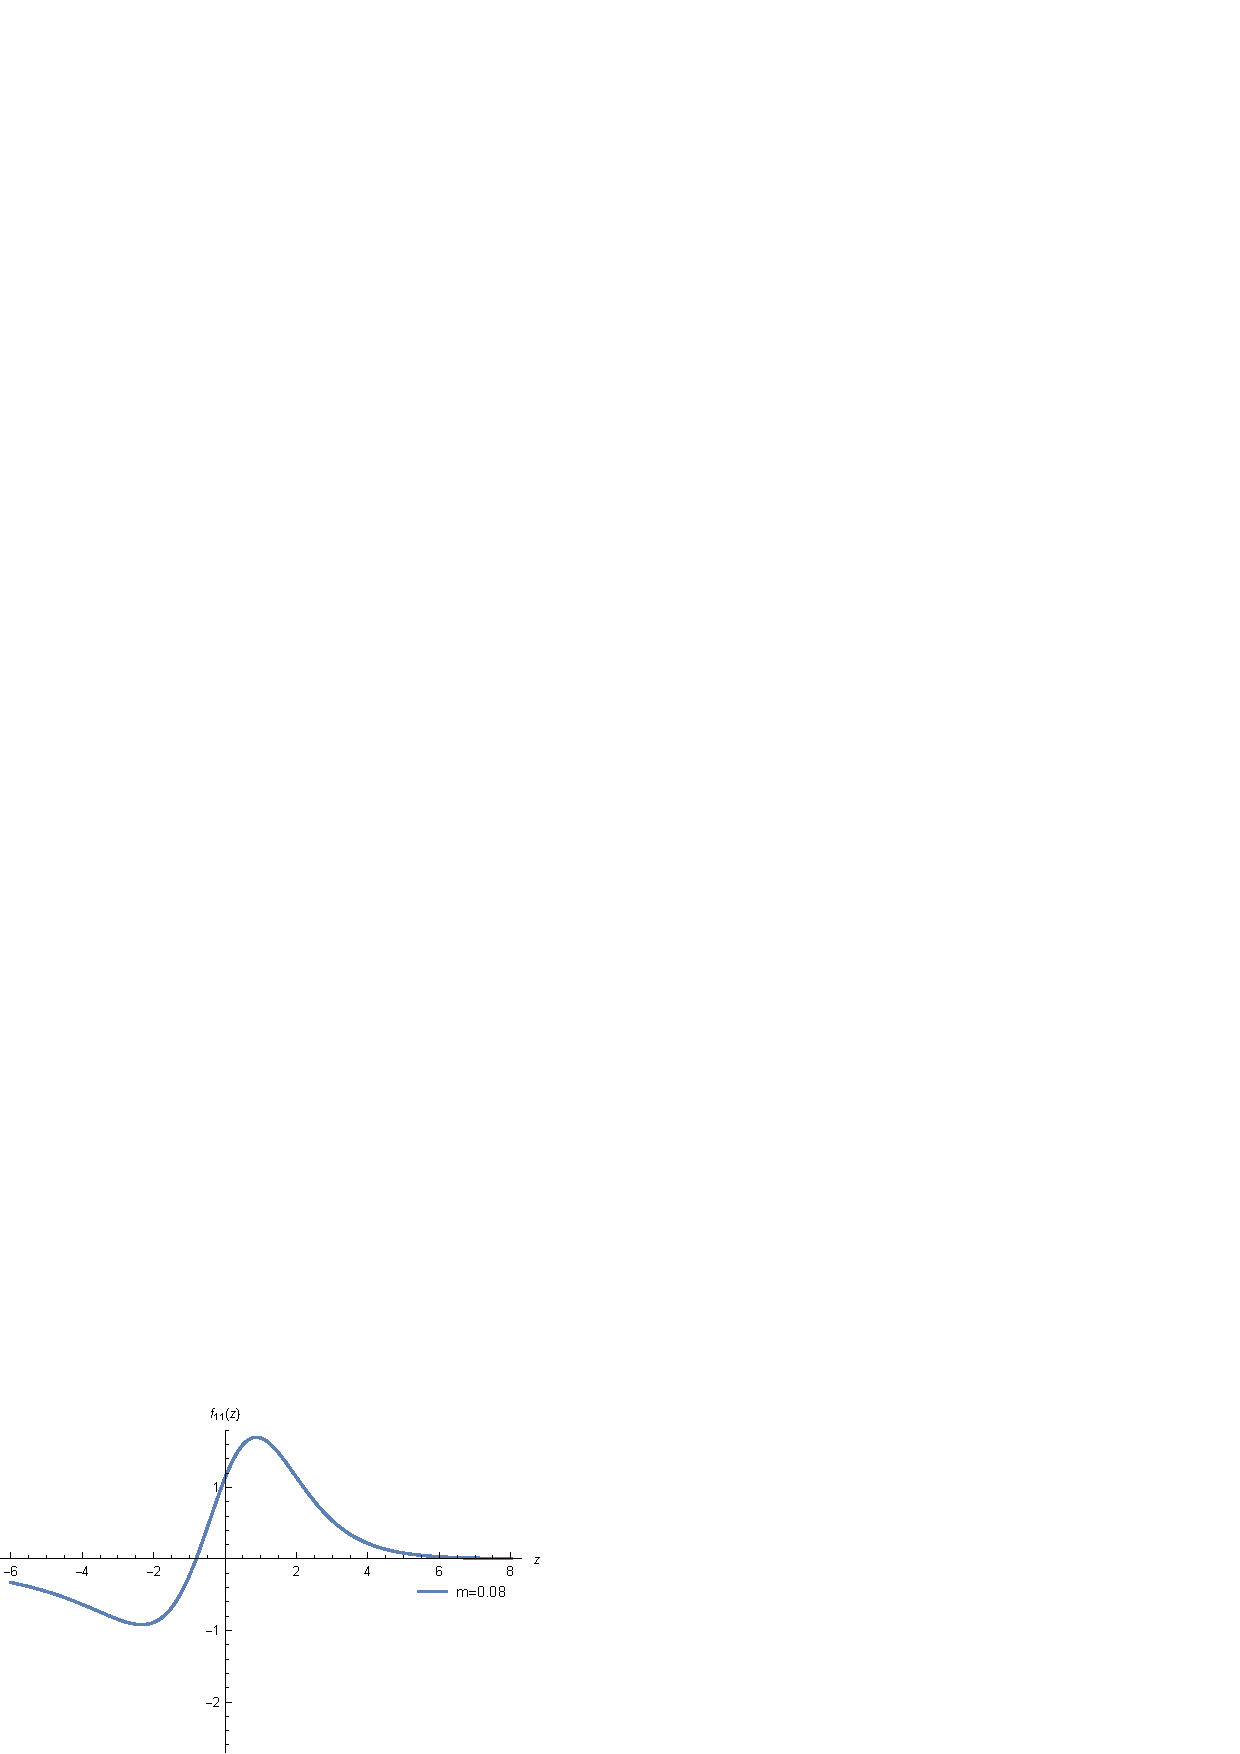
\includegraphics[width = 2.7in]{p008_before.pdf}} 
\subfloat[]{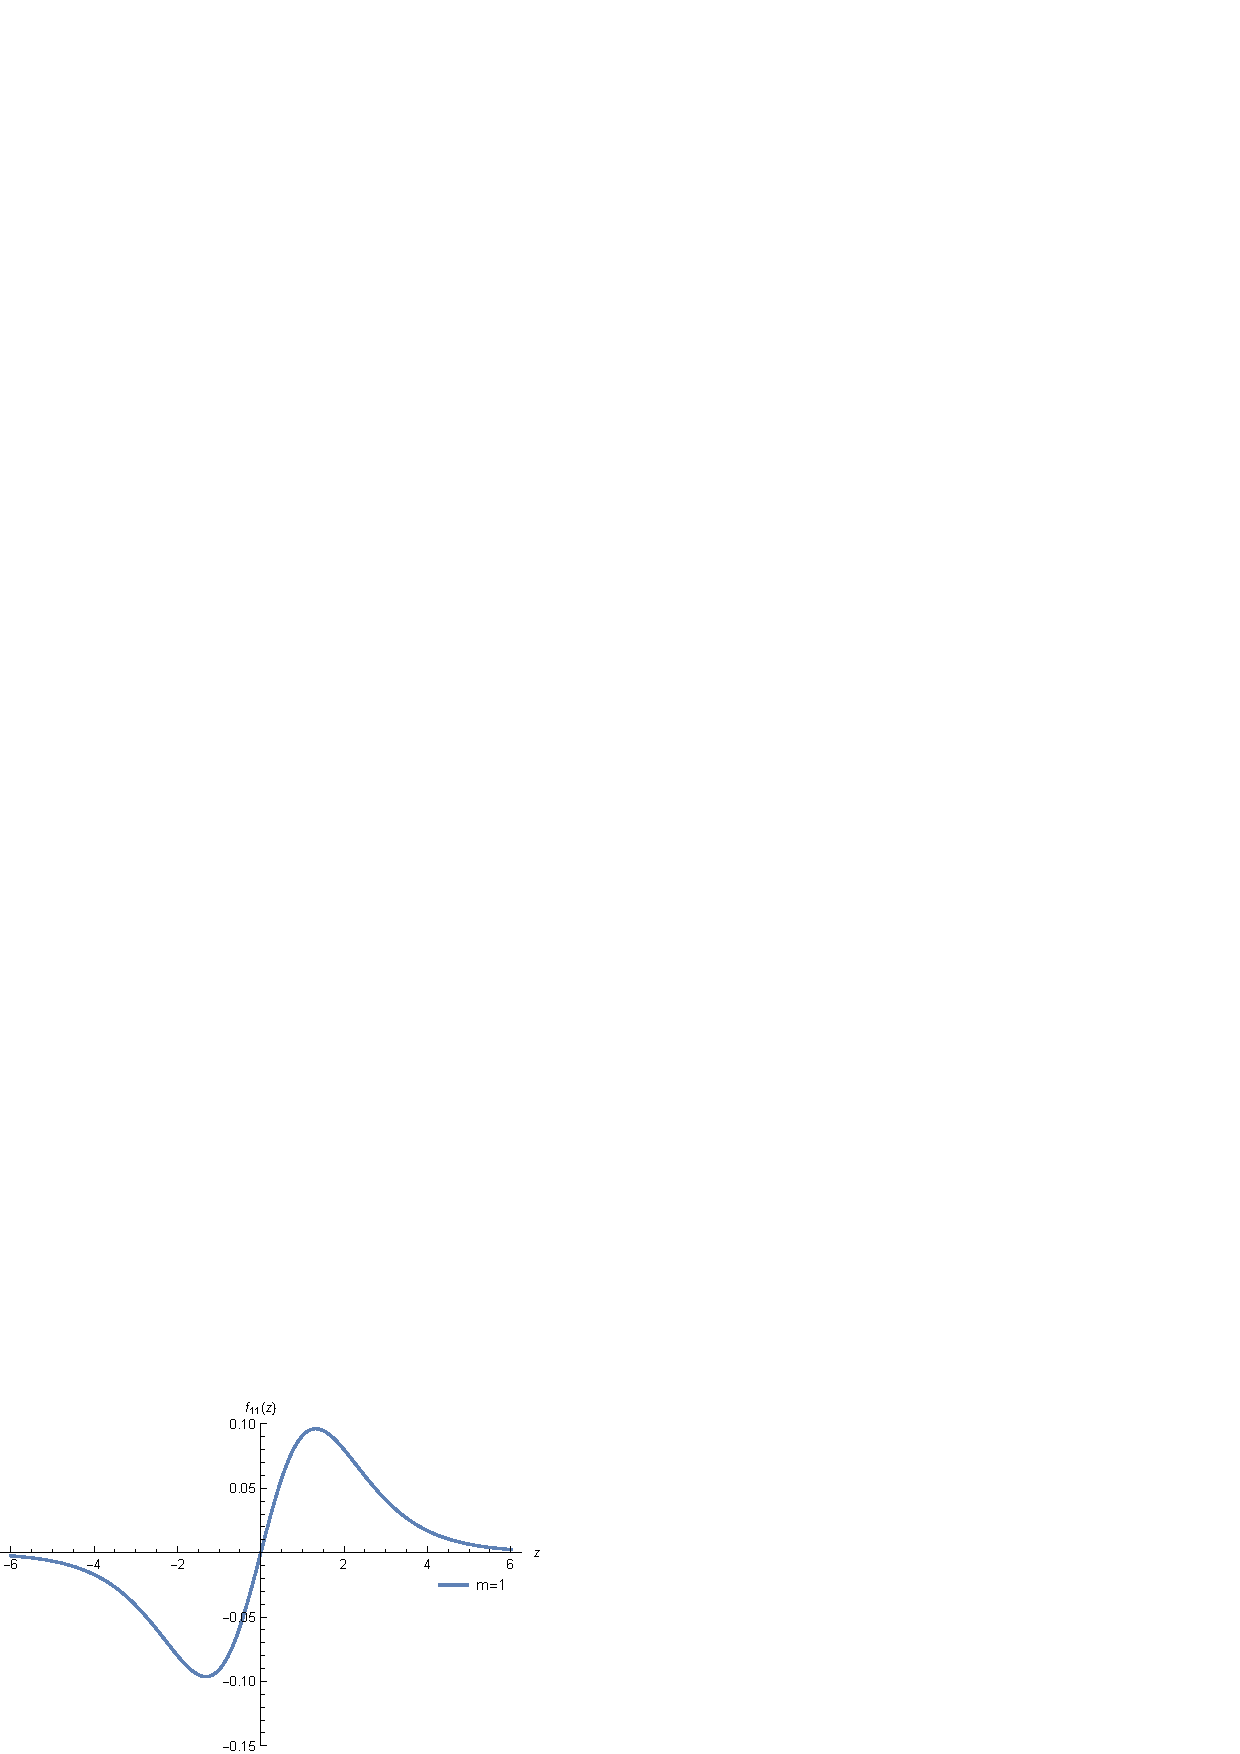
\includegraphics[width = 2.7in]{p1_before.pdf}}\\
\subfloat[]{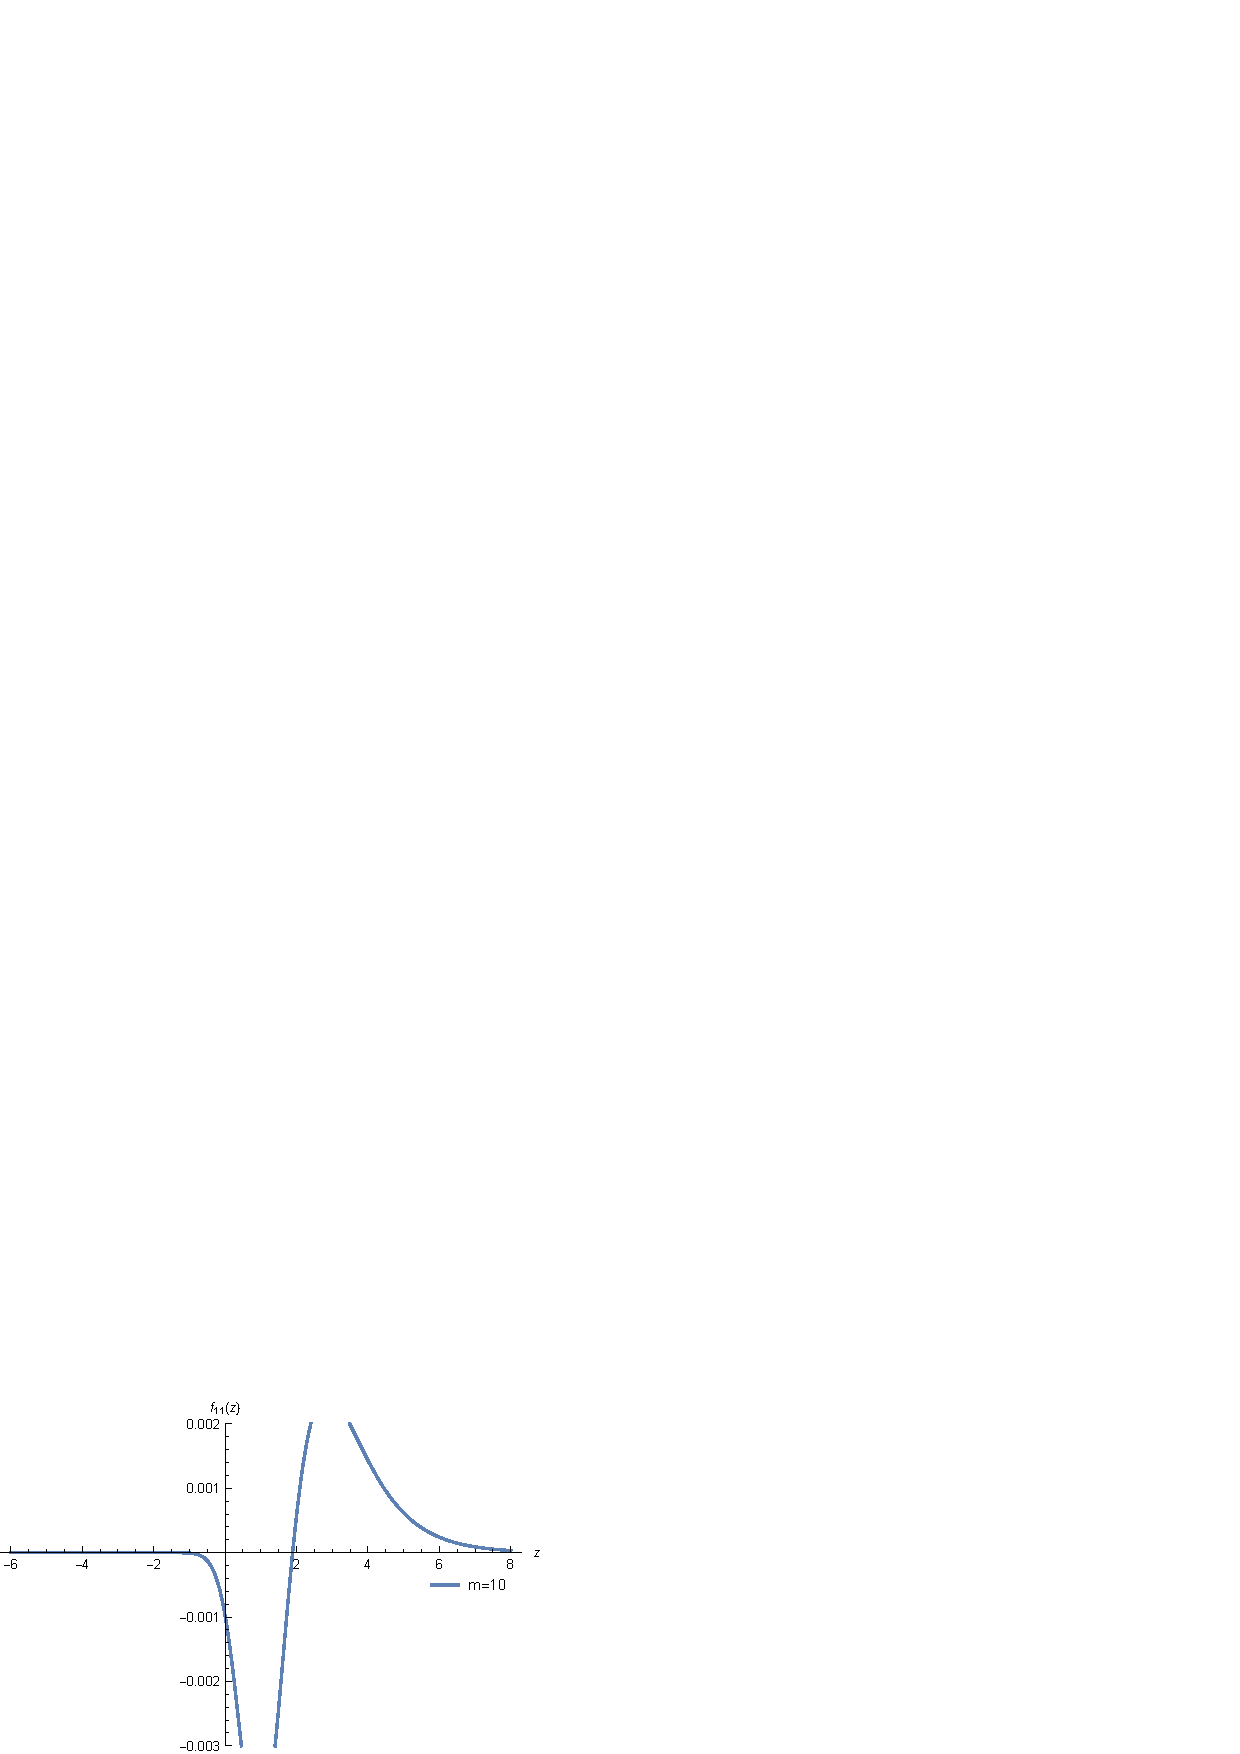
\includegraphics[width = 2.7in]{p10_before.pdf}}
\subfloat[]{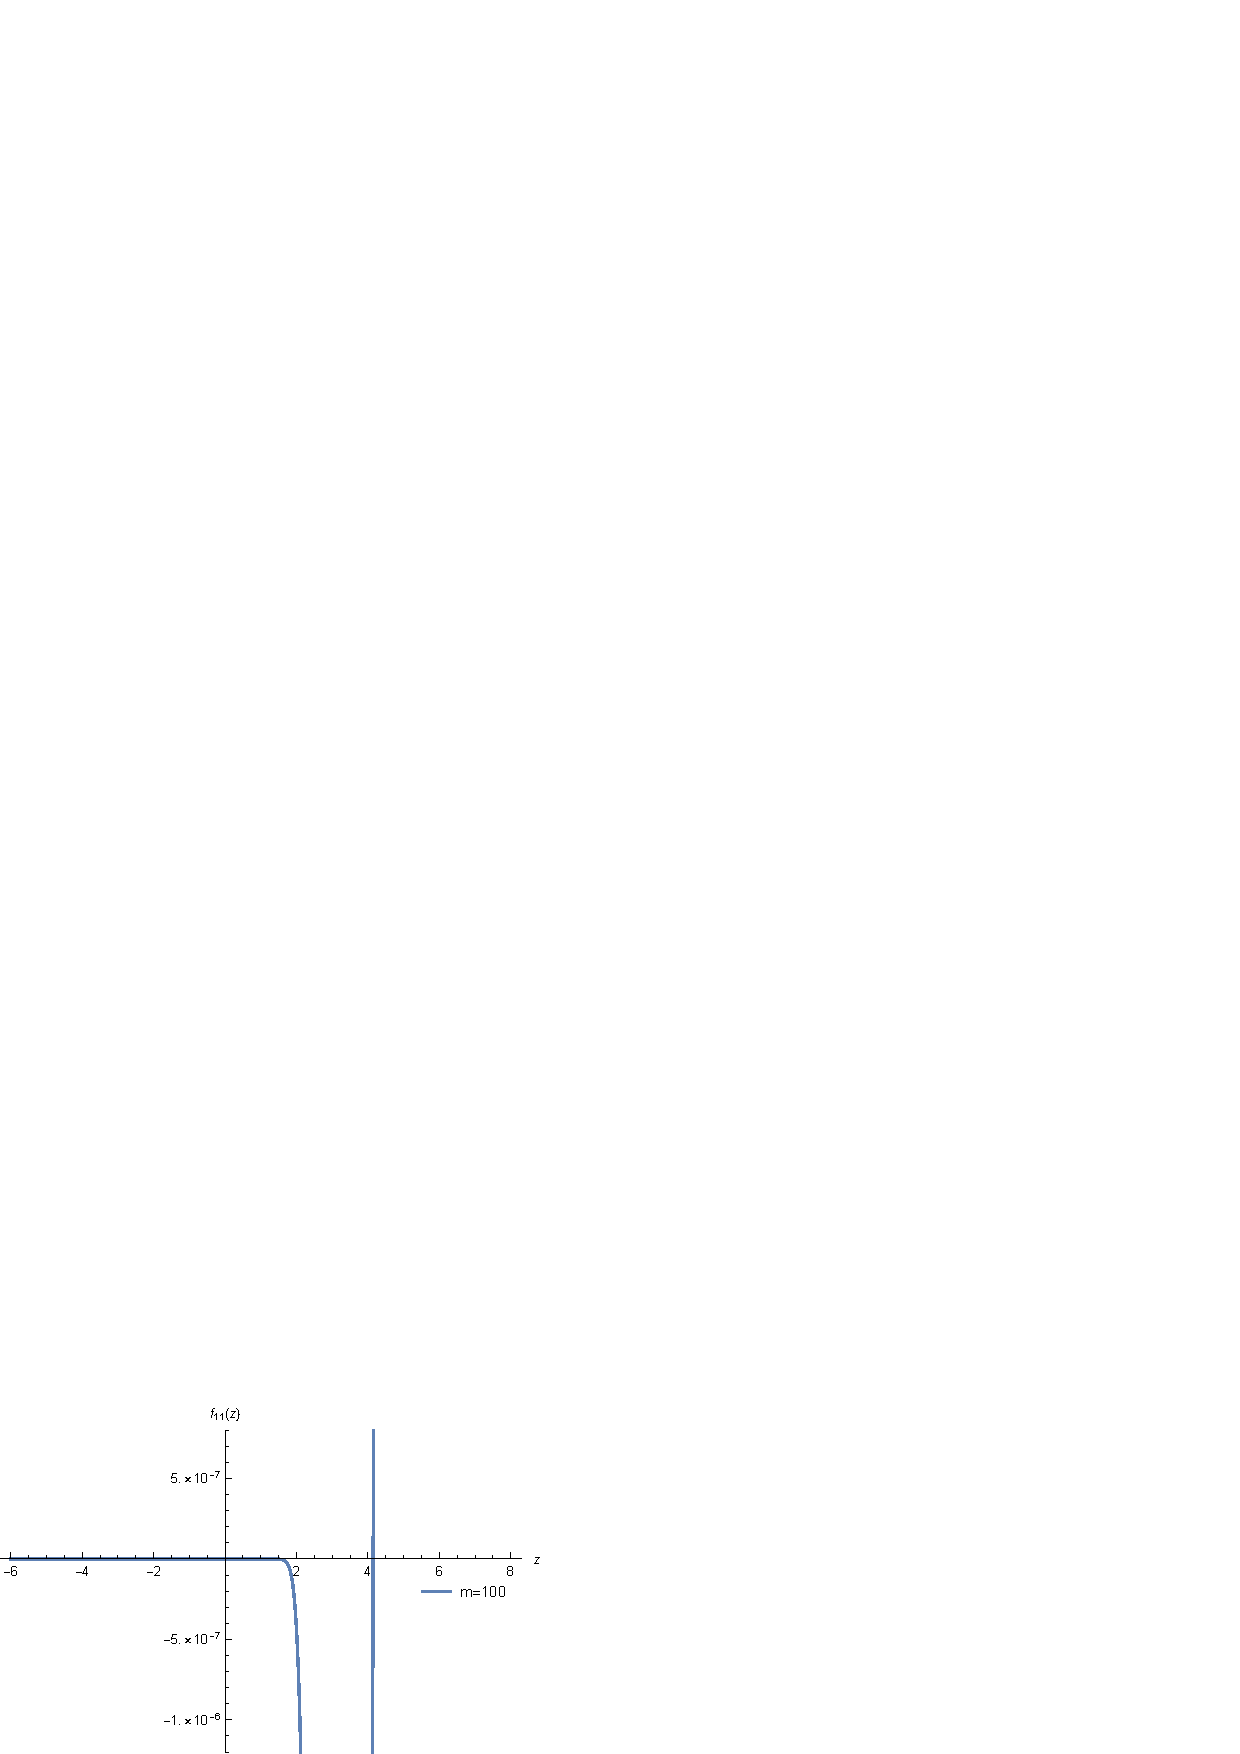
\includegraphics[width = 2.7in]{p100_before.pdf}} 
\caption{$f_{11}(z)$ for skewed logit model, z:[-6,8], m= 0.08,1,10, and 100}
\label{fig:skewedlogit_before}
\end{figure}
% Note that $g(z)>0$, therefore we can multiply all terms by $1/g(z)$. The sequence is now $\{1/g(z), 1,z, z^2\}$. By definition of T-system and matrix algebra, we have work instead with $\{1,z, z^2,-1/g(z)\}$. 


% We will continue with 2 of \ref{proc} and add $e^z$ to the sequence.
To resolve this issue, we insert an ancillary function $e^zg(z)$ to $S_1$, and divide all terms by $g(z)$. After proper permutation, the new sequence contains $\Psi_0(z) = 1$, $\Psi_1(z) = z$, $\Psi_2(z) = z^2$,  $\Psi_3(z) = e^z$, and $\Psi_4(z) =- (1+e^z)^2(-1+(1+e^{-z})^m)$.
Calculation shows $f_{1,1}(z) = 1$, $f_{2,2}(z) =2$, and $f_{3,3}(z) = e^z/2$. The last function $f_{4,4}(z)$ has a complicated form, and the value depends on $m$ for $z\in (-\infty, \infty)$. Specifically, numeric results show that $f_{4,4}(z)<0$ for  $z\in (-\infty, \infty)$ when $m\ge 0.2$.
\begin{figure}[ht]
\subfloat[]{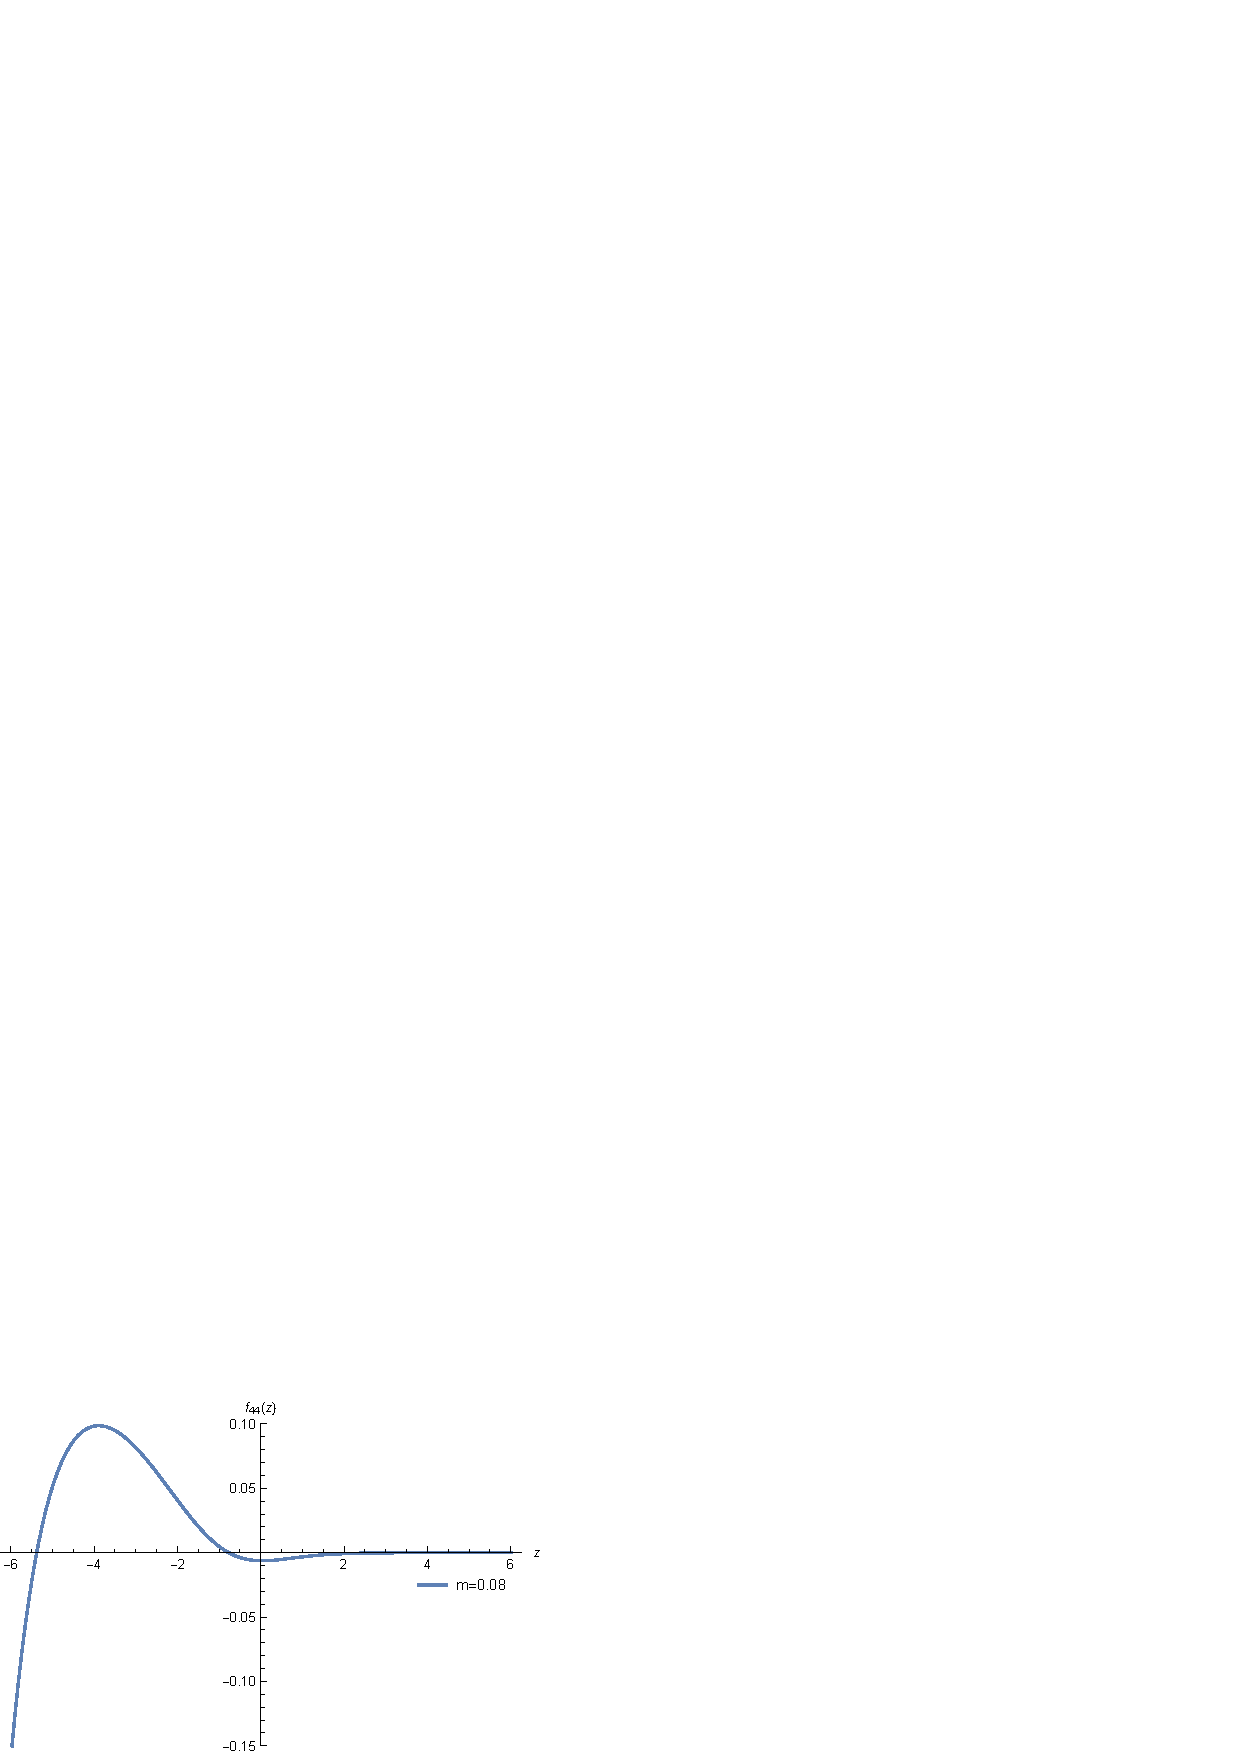
\includegraphics[width = 2.7in]{p008.pdf}} 
\subfloat[]{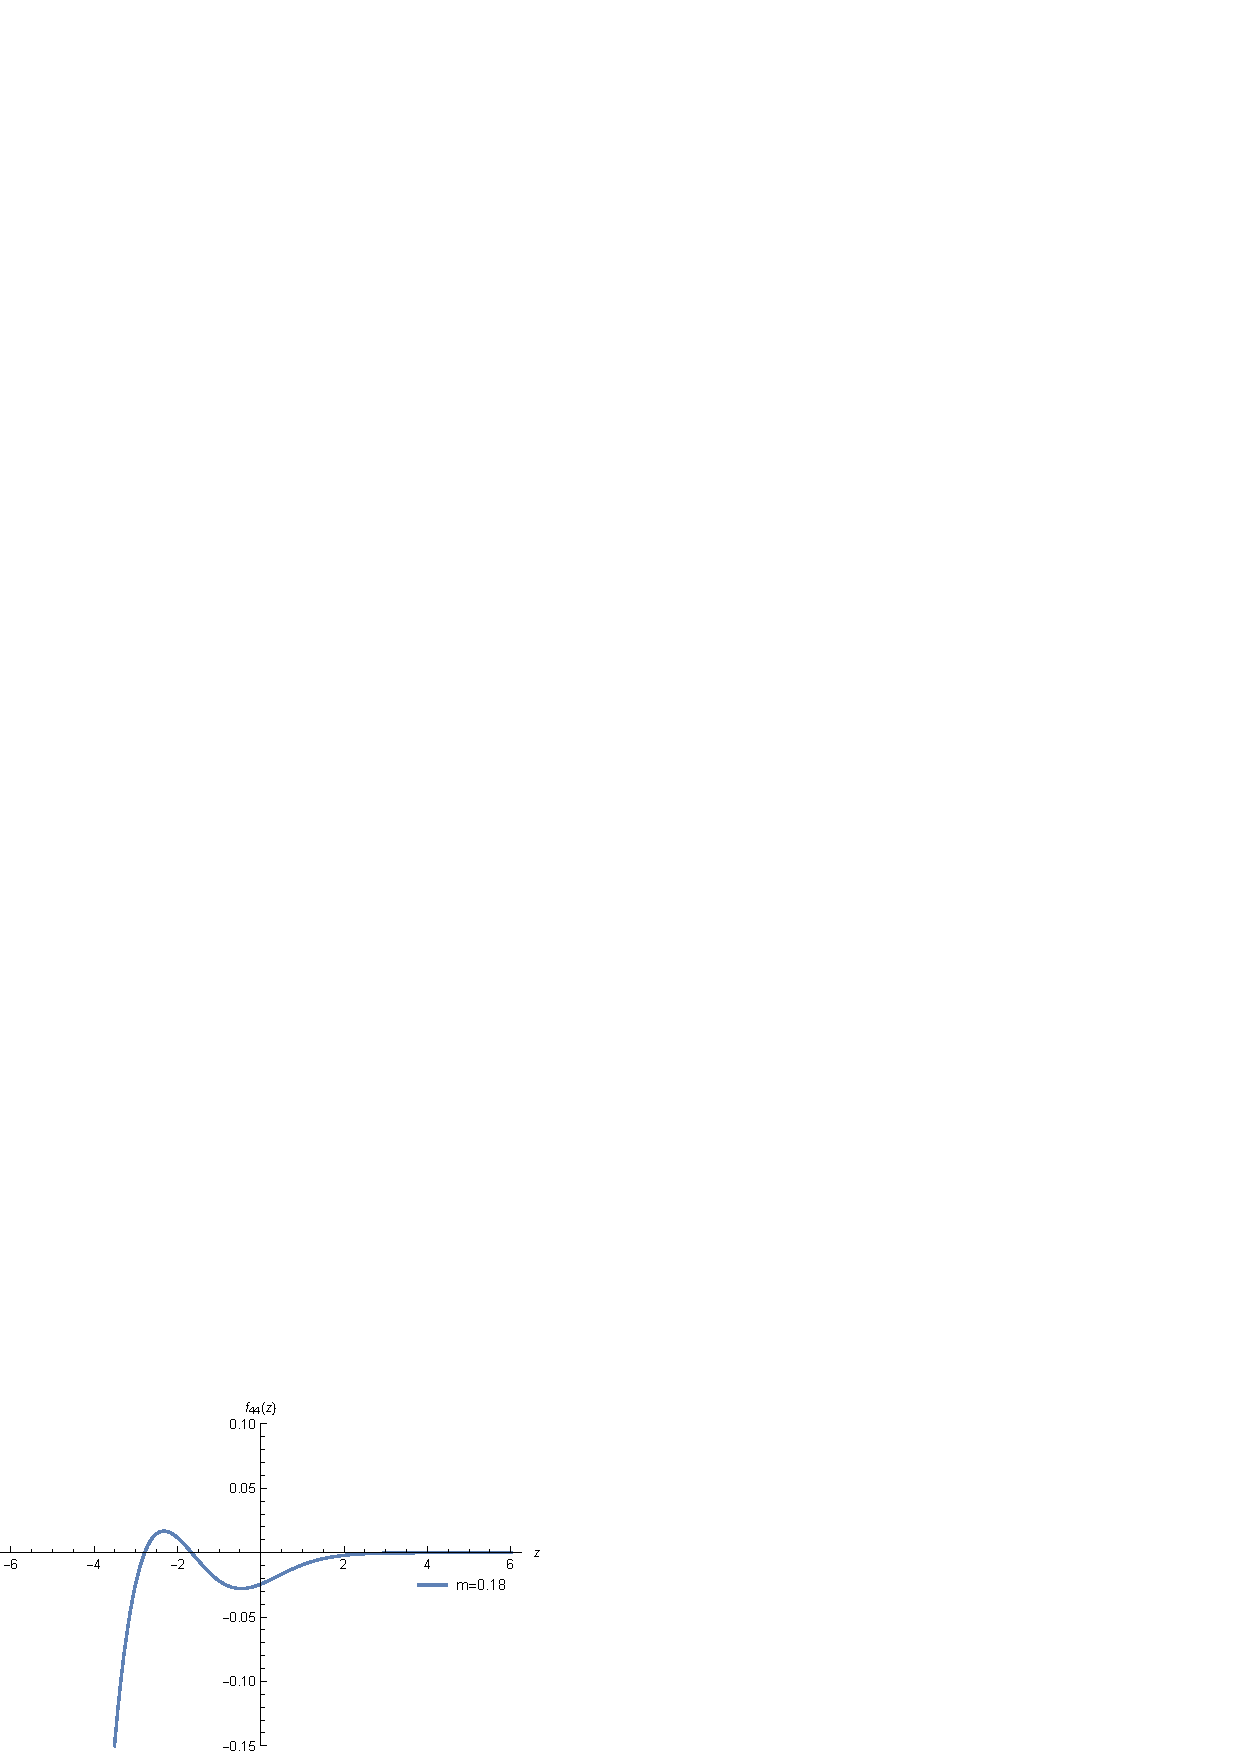
\includegraphics[width = 2.7in]{p018.pdf}} \\
\subfloat[]{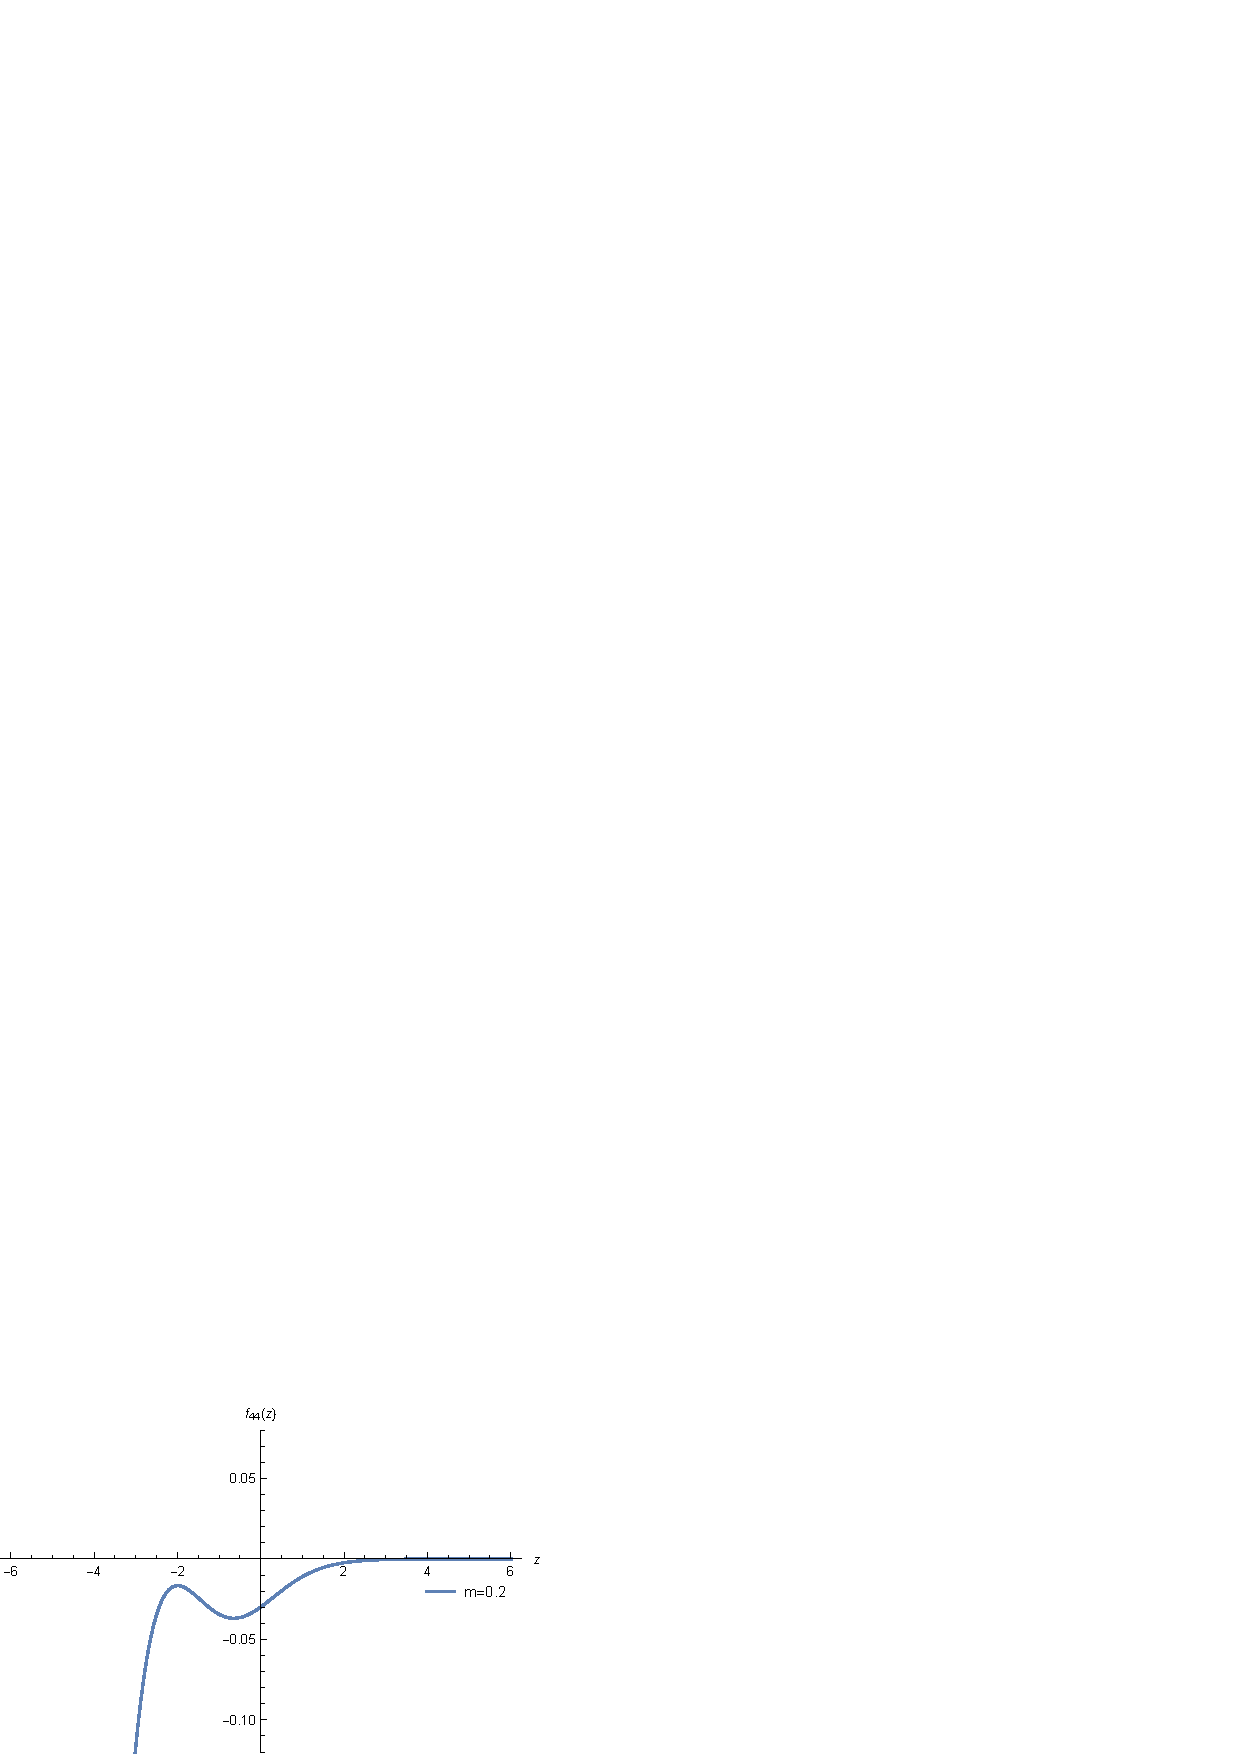
\includegraphics[width = 2.7in]{p02.pdf}} 
\subfloat[]{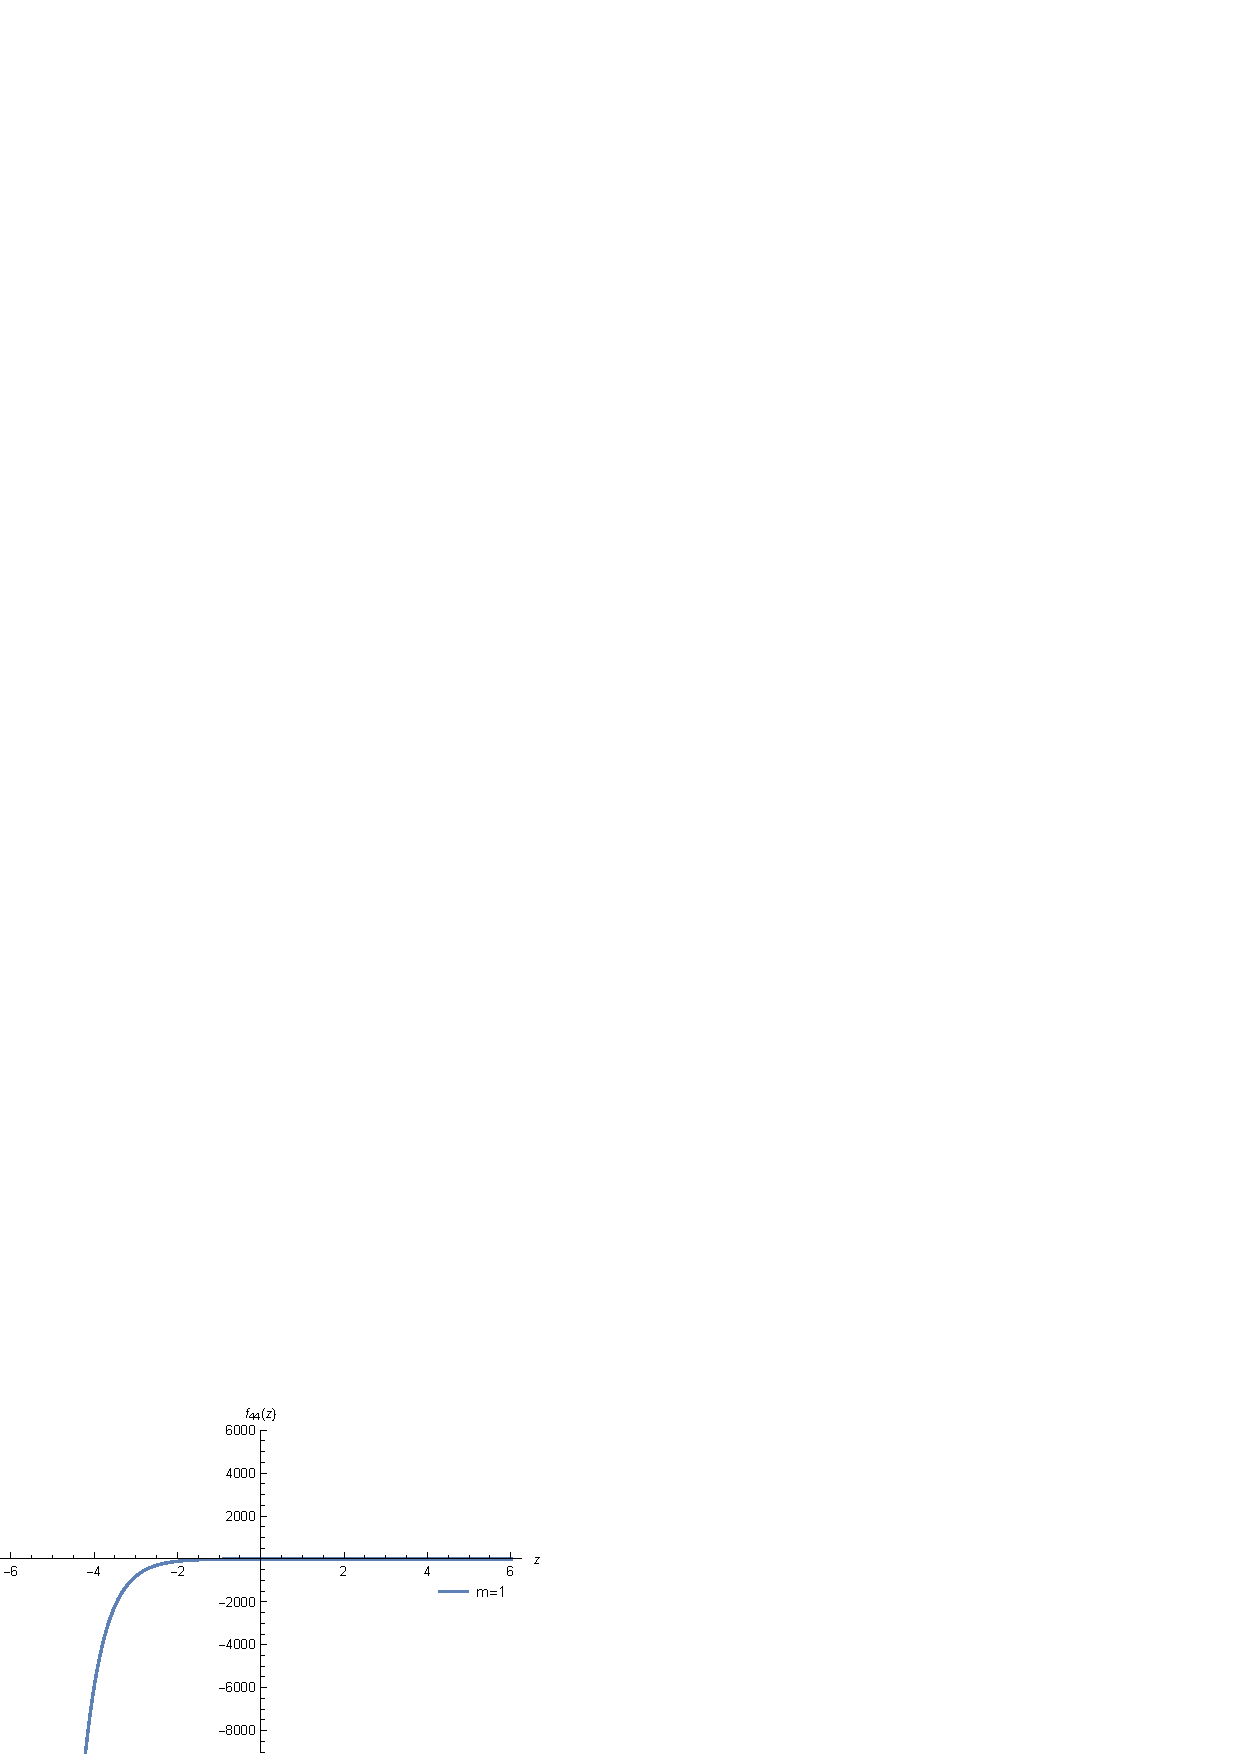
\includegraphics[width = 2.7in]{p1.pdf}}\\
\subfloat[]{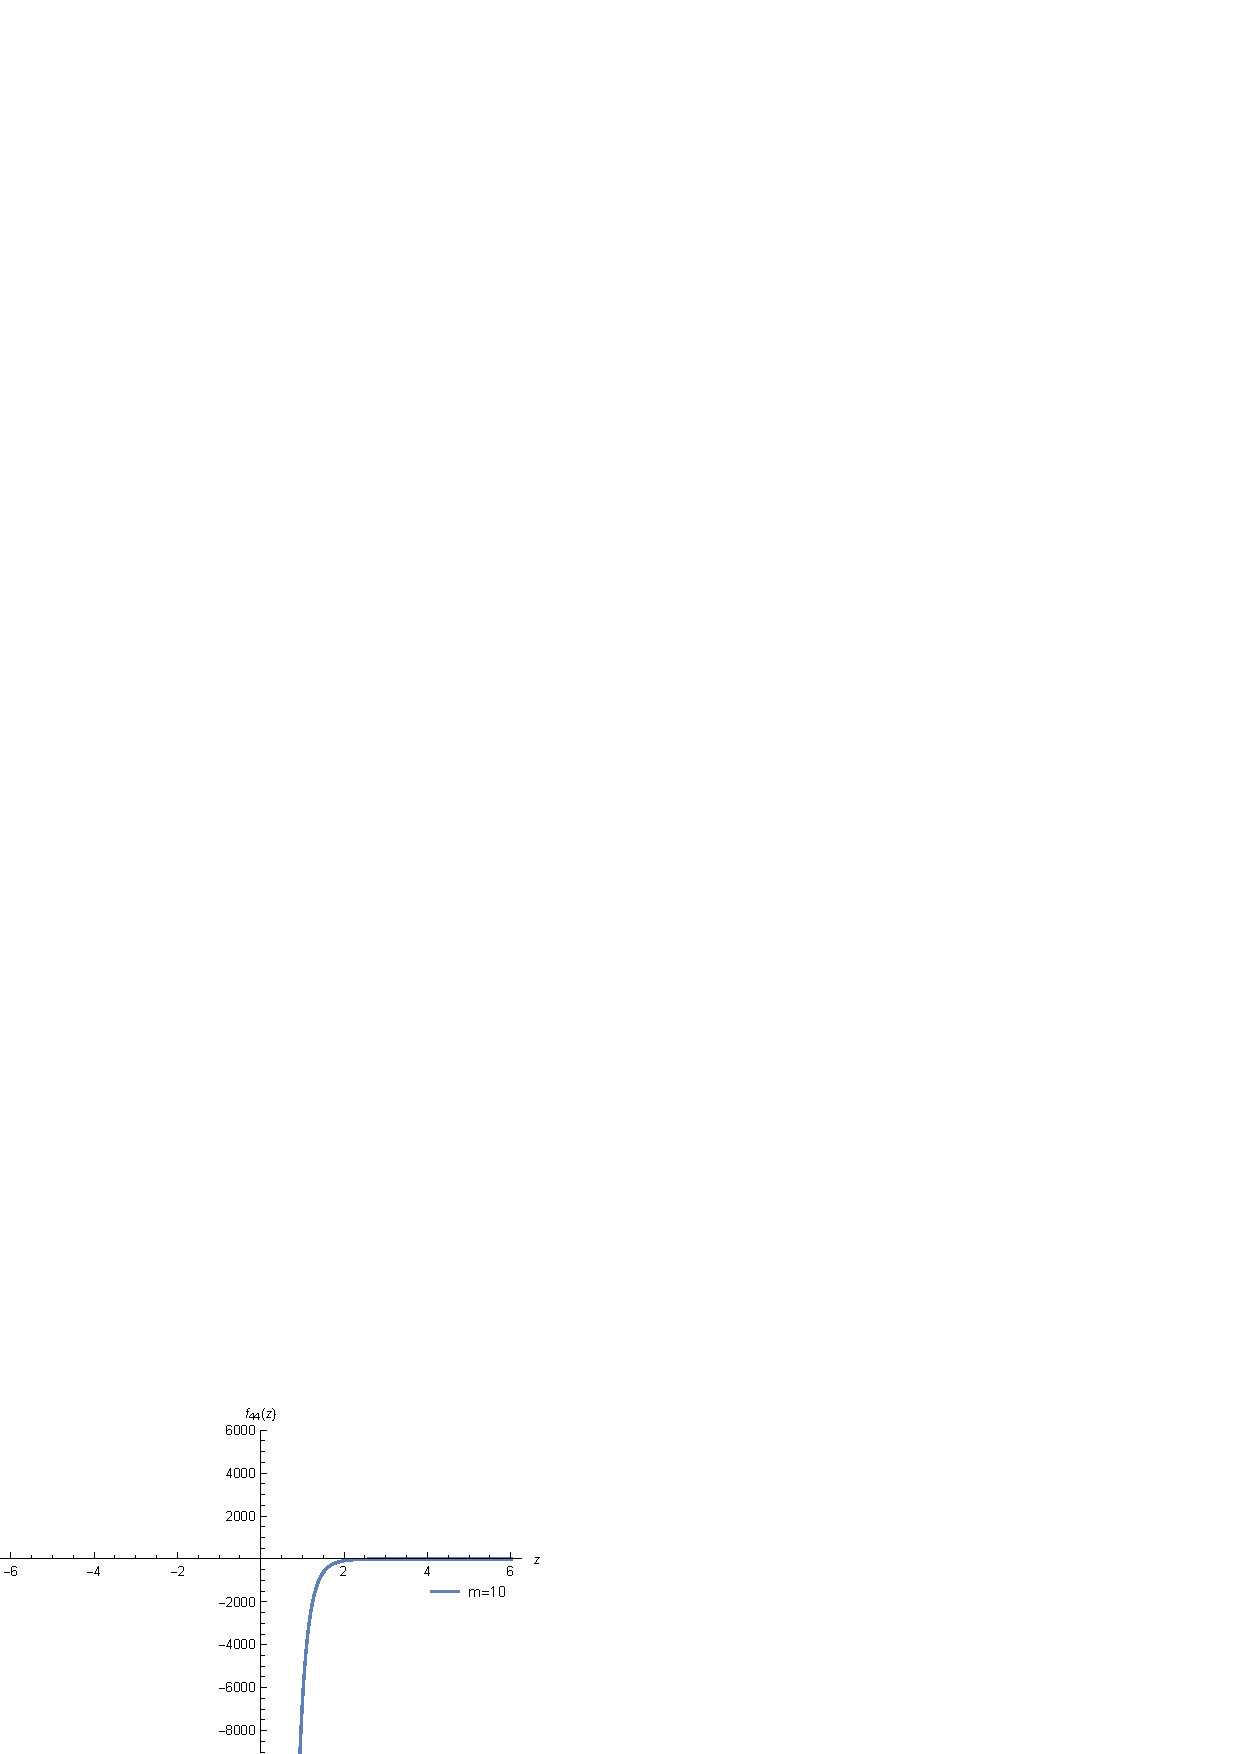
\includegraphics[width = 2.7in]{p10.pdf}}
\subfloat[]{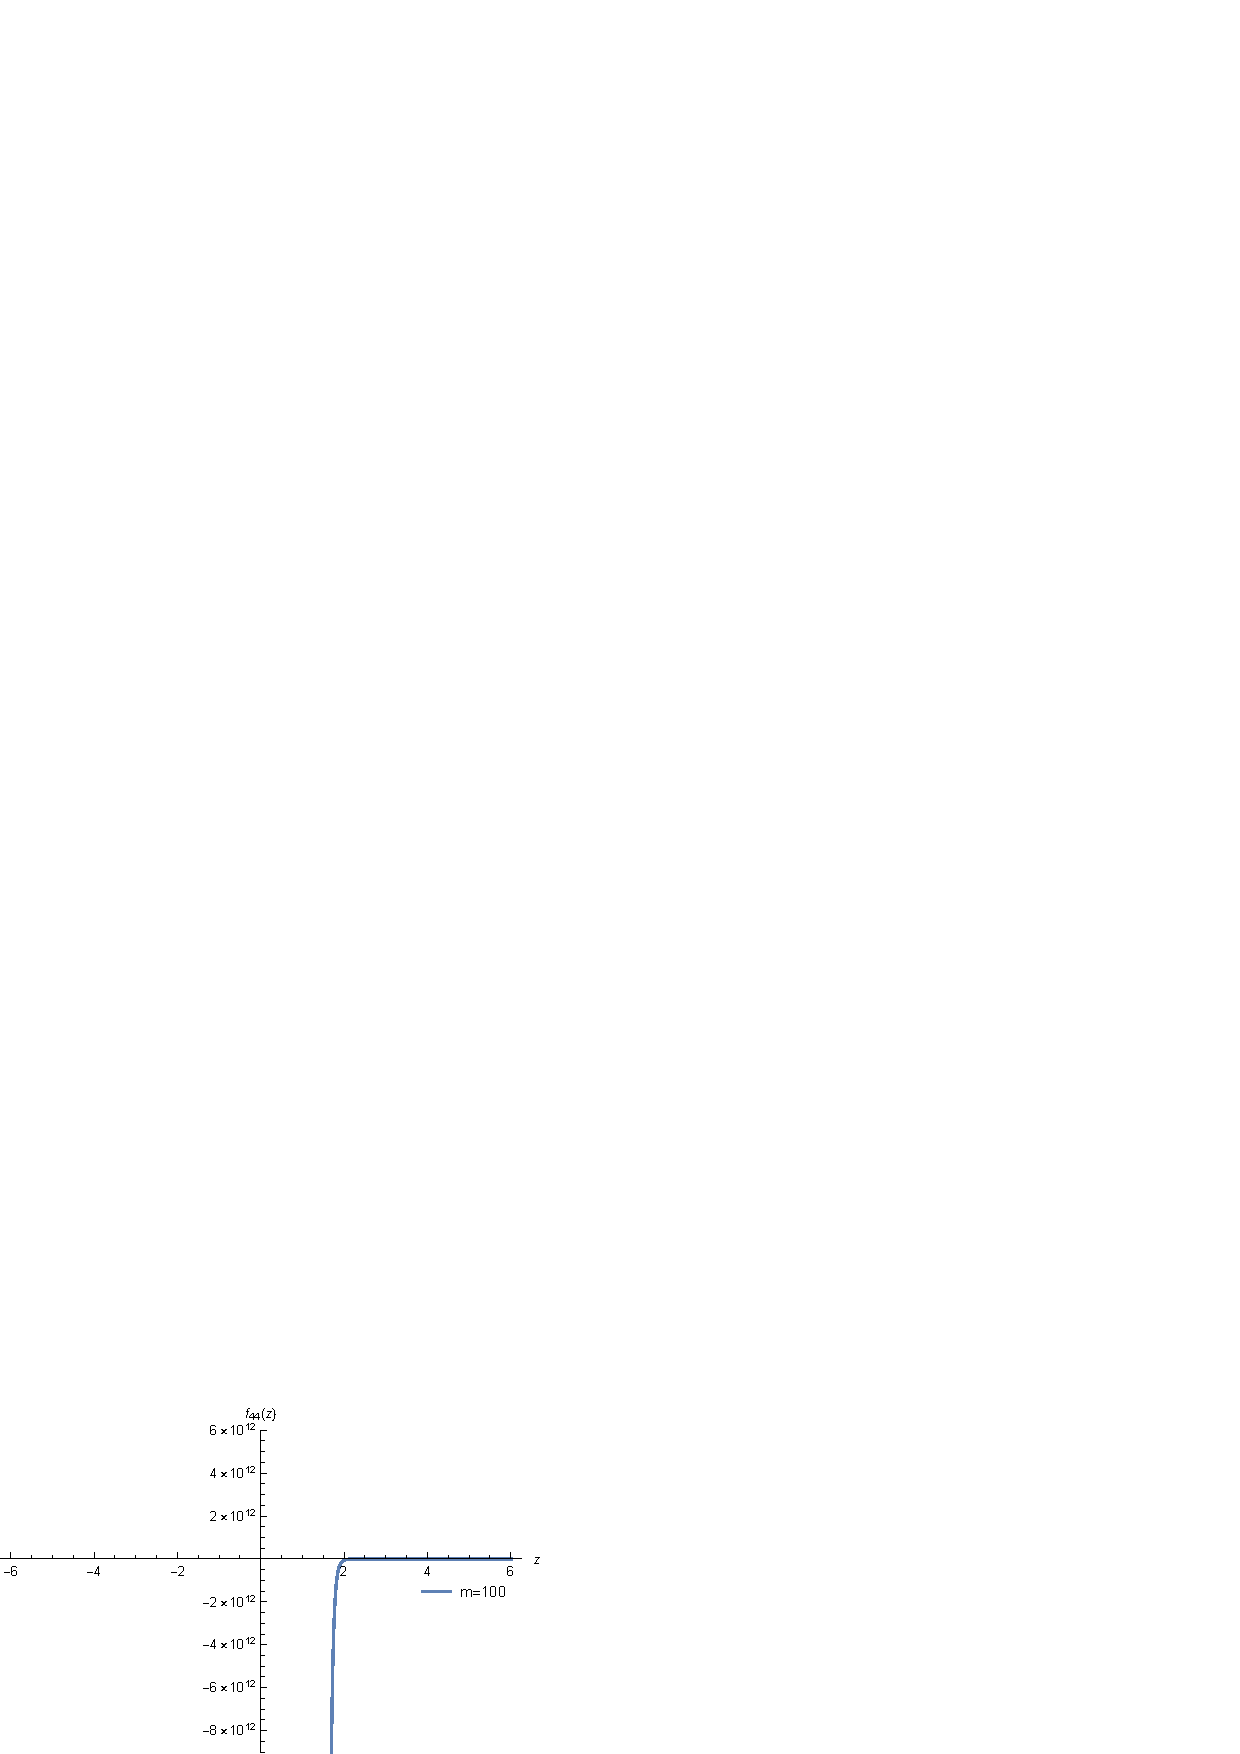
\includegraphics[width = 2.7in]{p100.pdf}} 
\caption{$f_{44}(z)$ for skewed logit model, z:[-6,6], m= 0.08, 0.18, 0.2,1,10, and 100}
\label{fig:skewedlogit_after}
\end{figure}

\begin{figure}[ht]
\subfloat[]{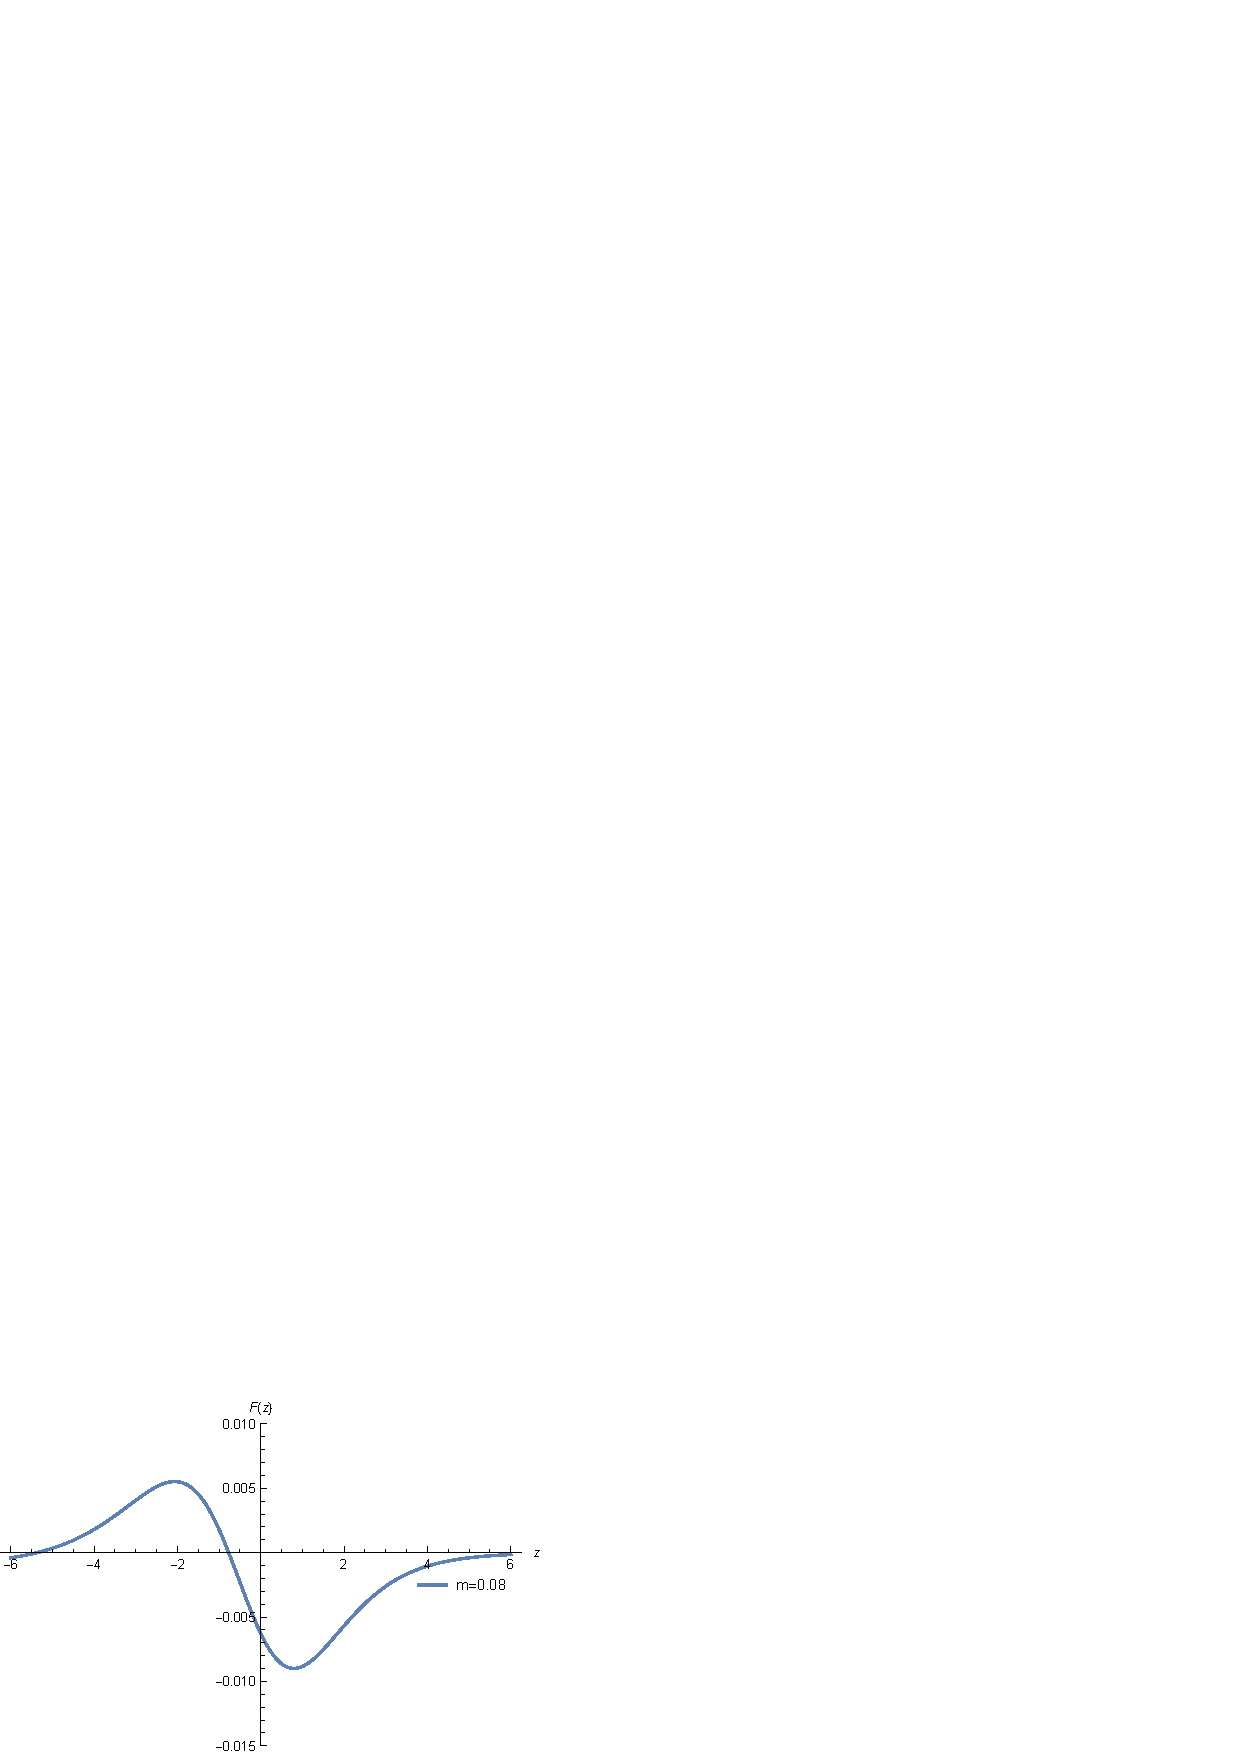
\includegraphics[width = 2.7in]{p008_F.pdf}} 
\subfloat[]{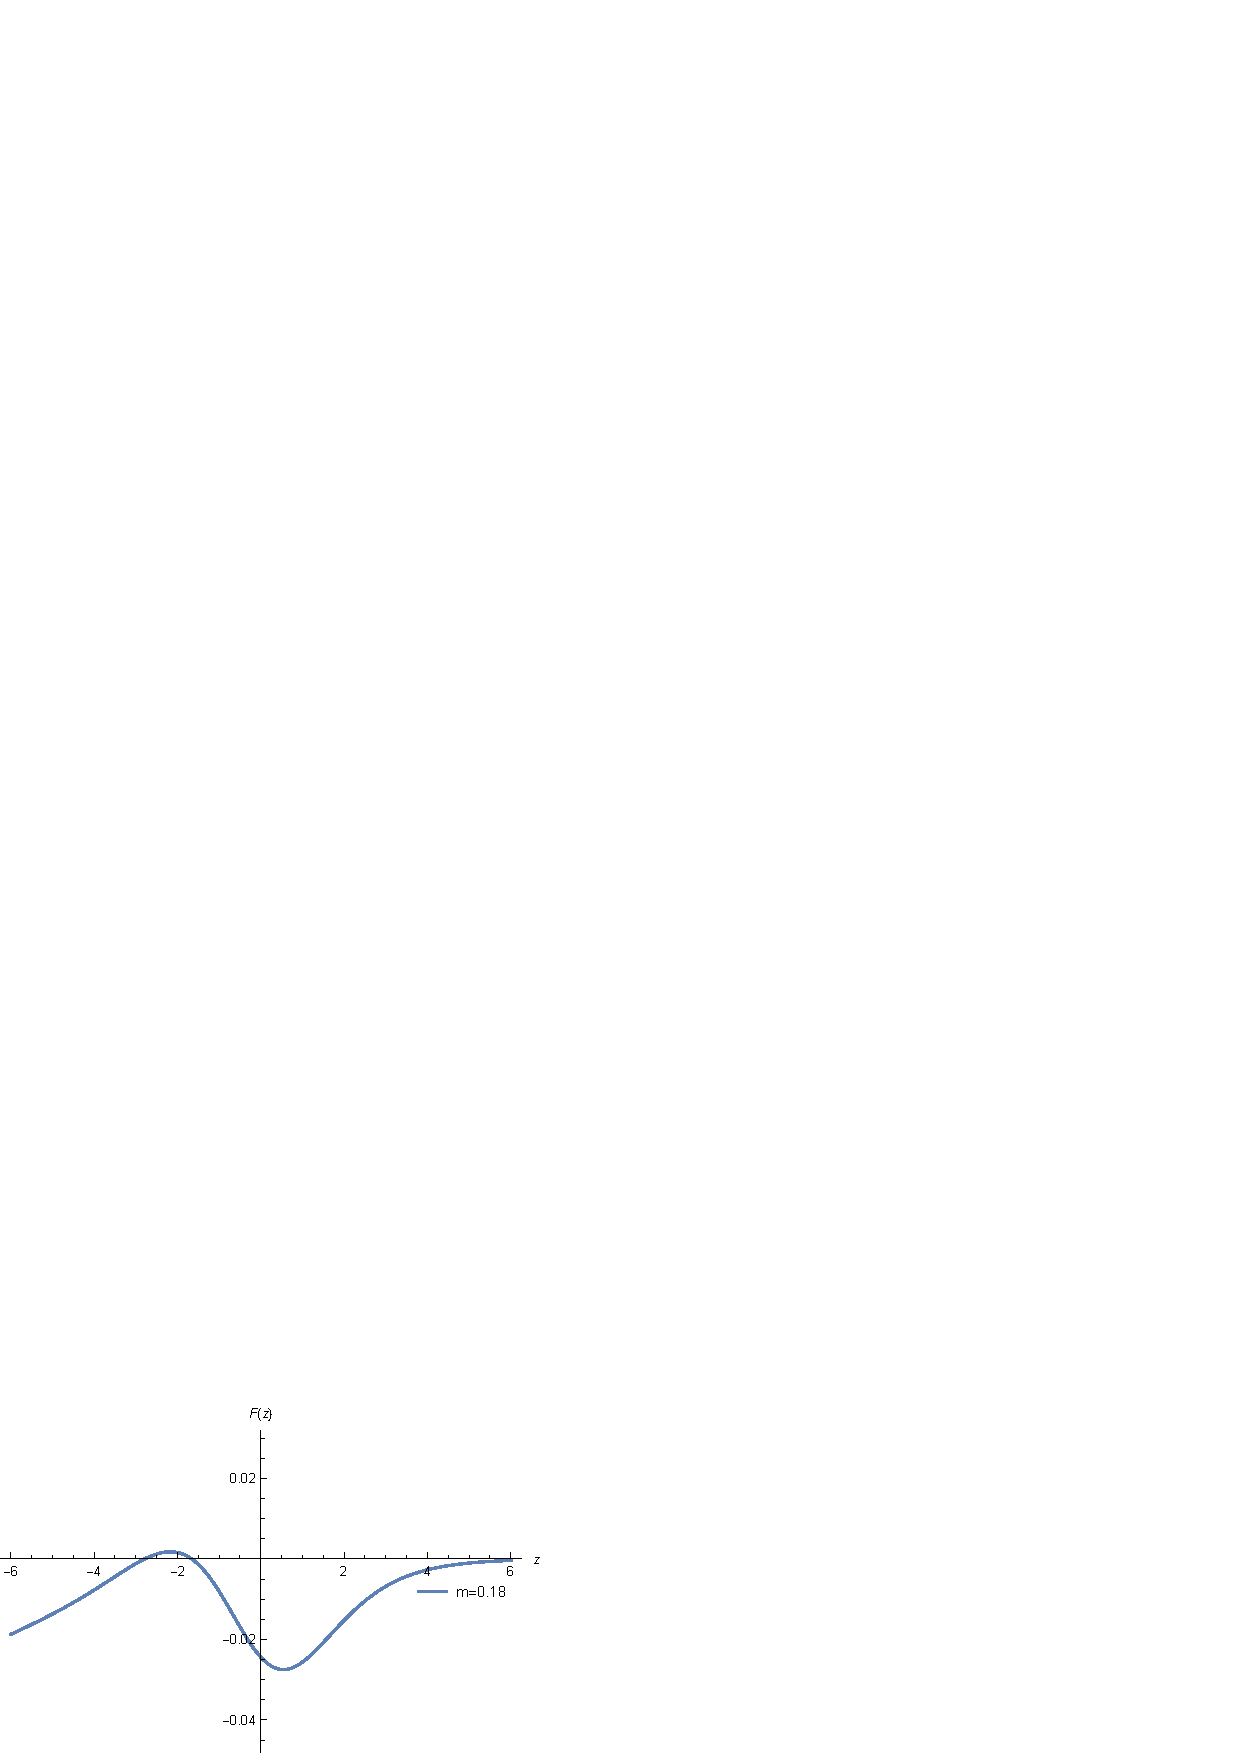
\includegraphics[width = 2.7in]{p018_F.pdf}} \\
\subfloat[]{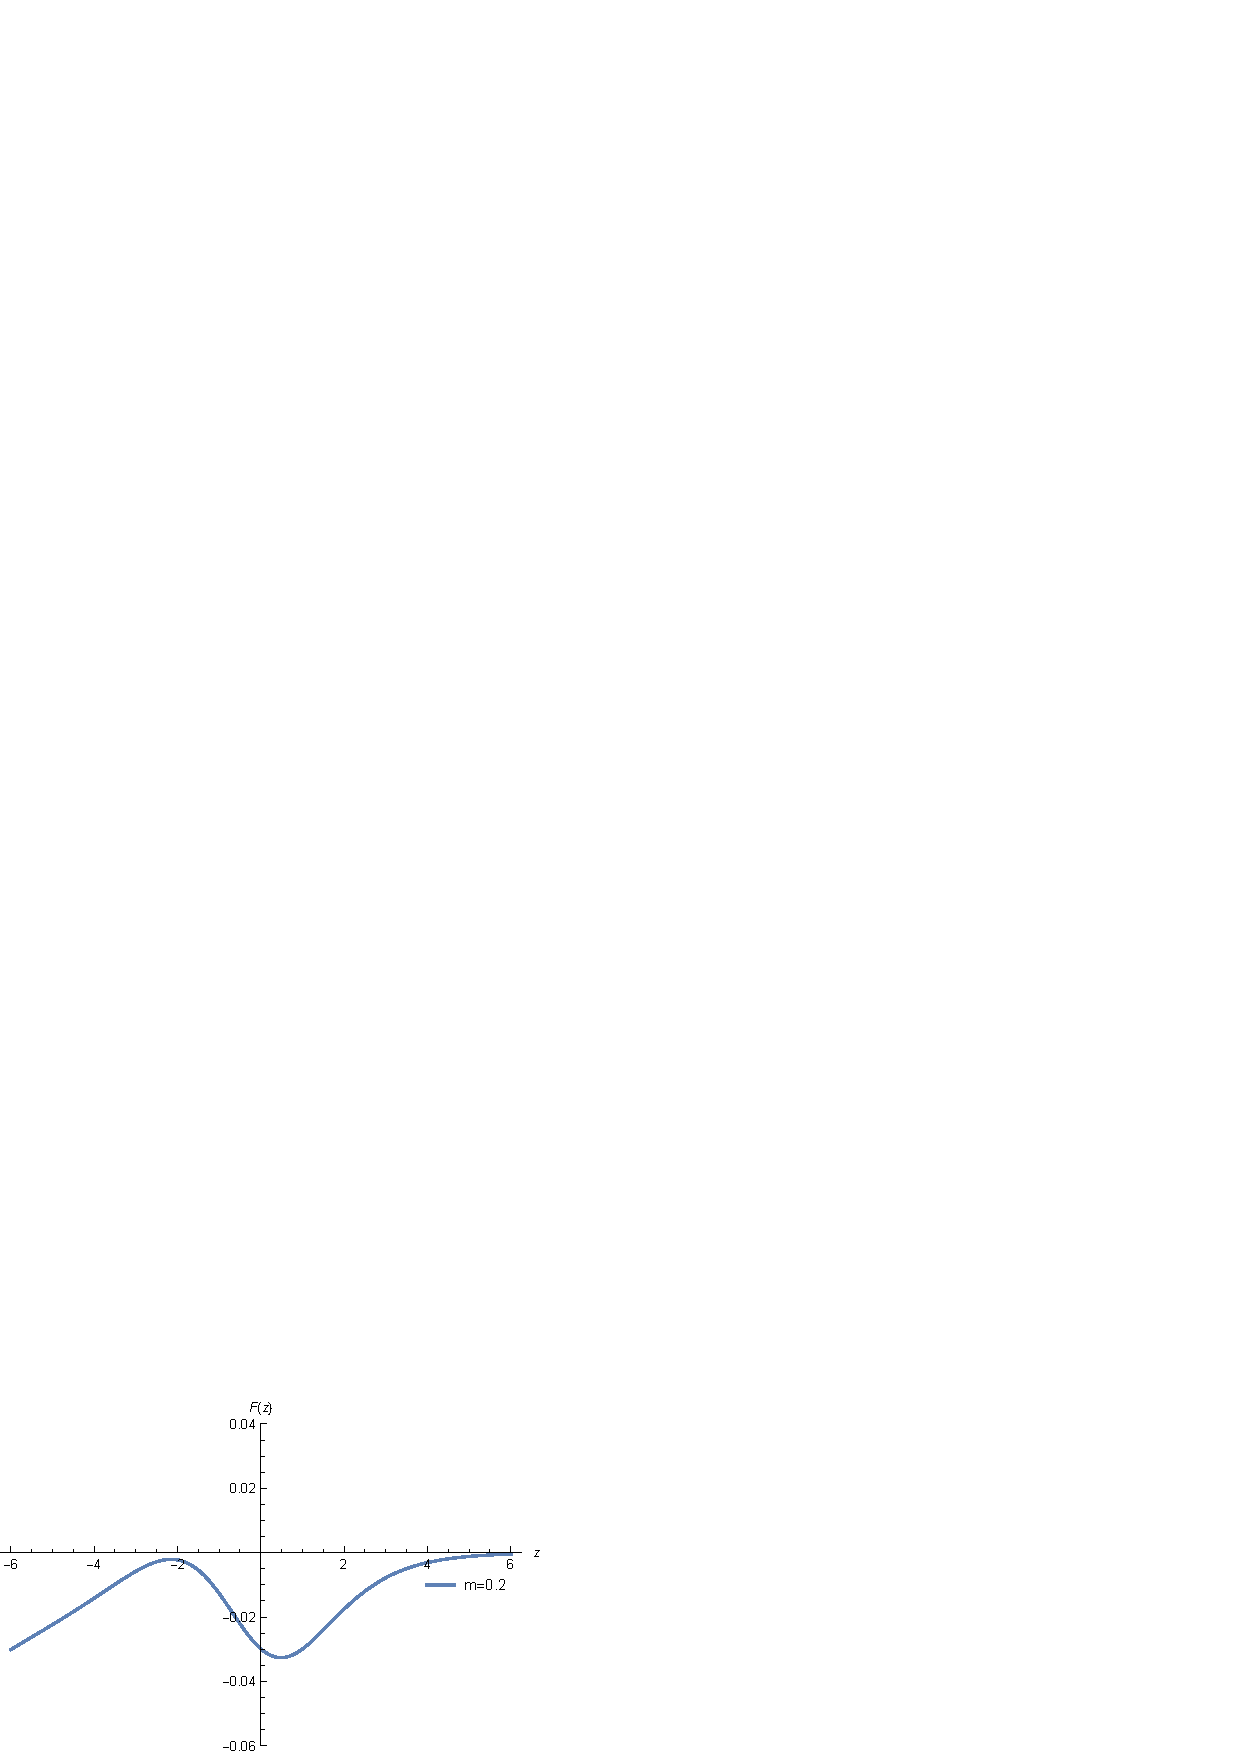
\includegraphics[width = 2.7in]{p02_F.pdf}} 
\subfloat[]{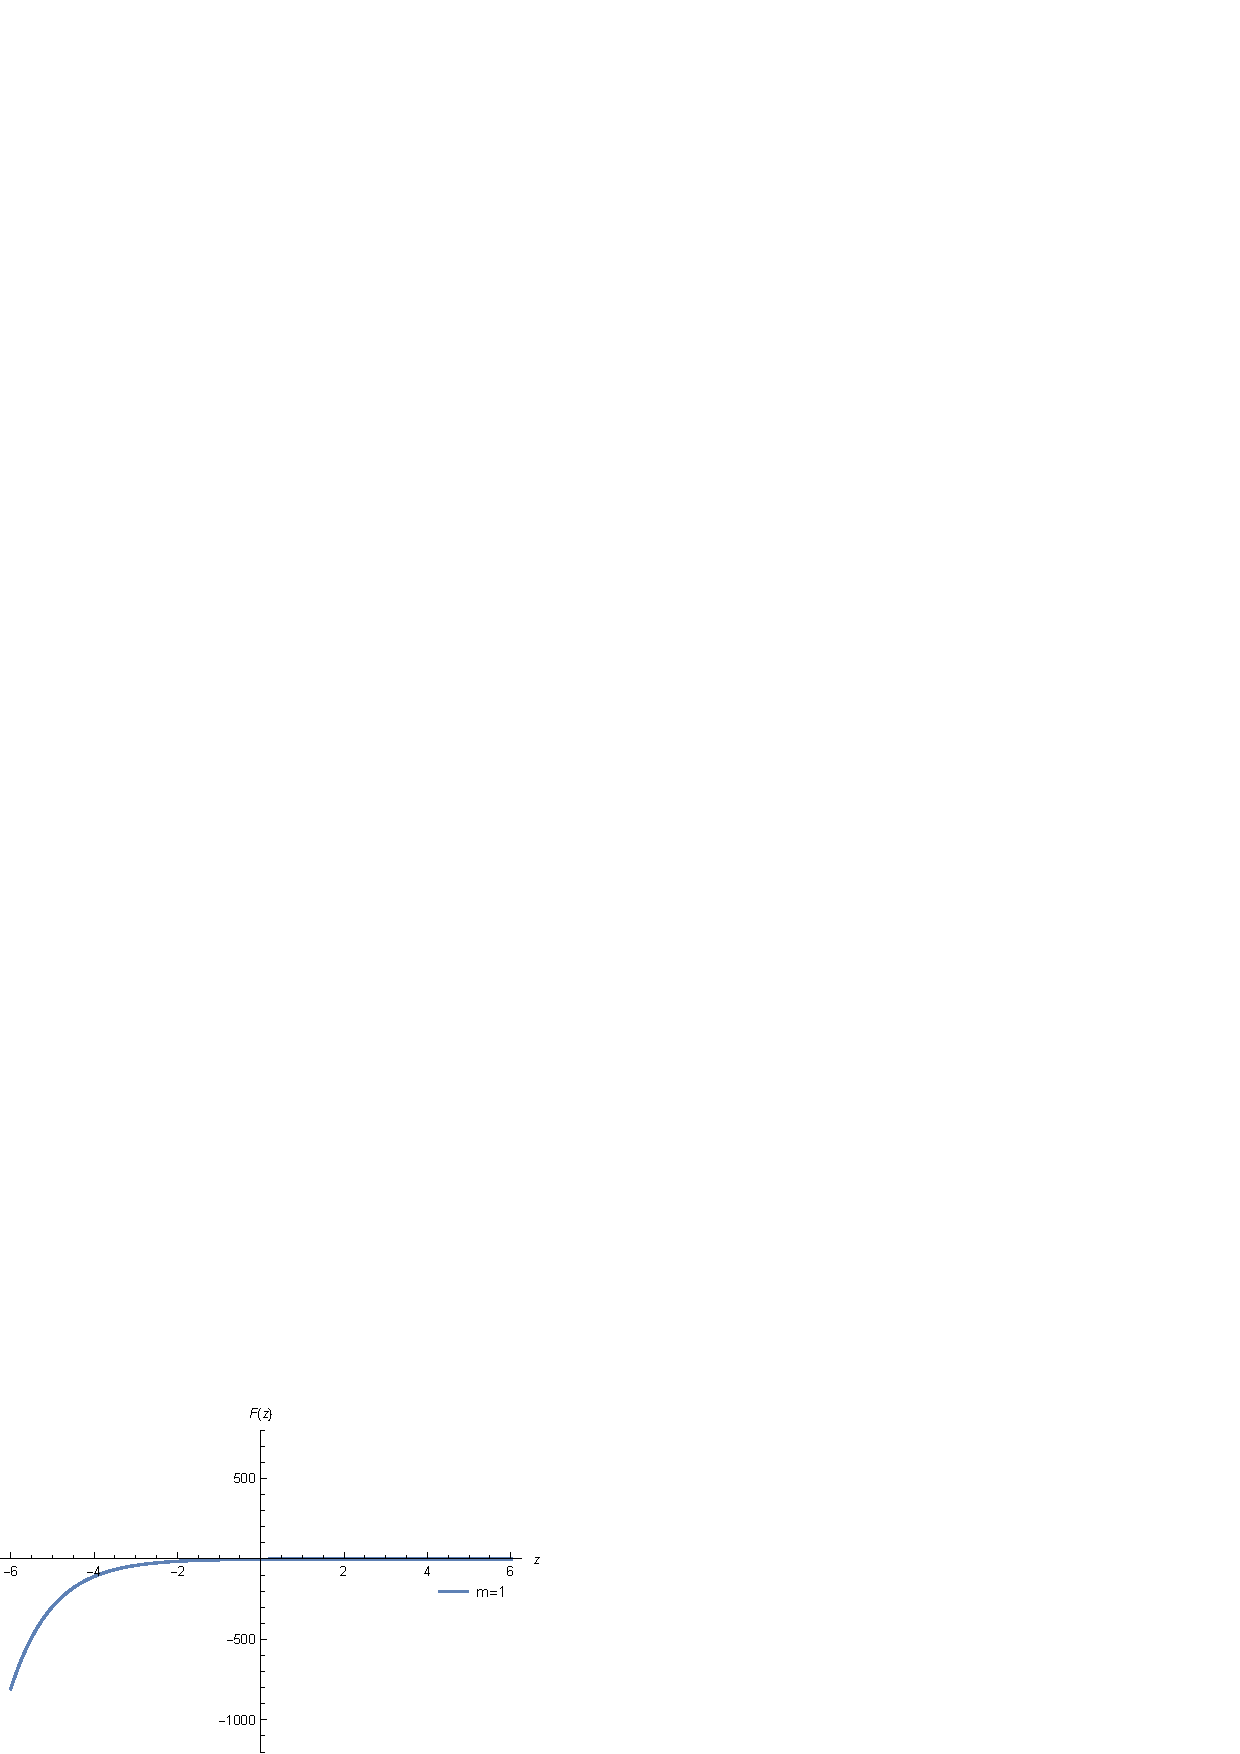
\includegraphics[width = 2.7in]{p1_F.pdf}}\\
\subfloat[]{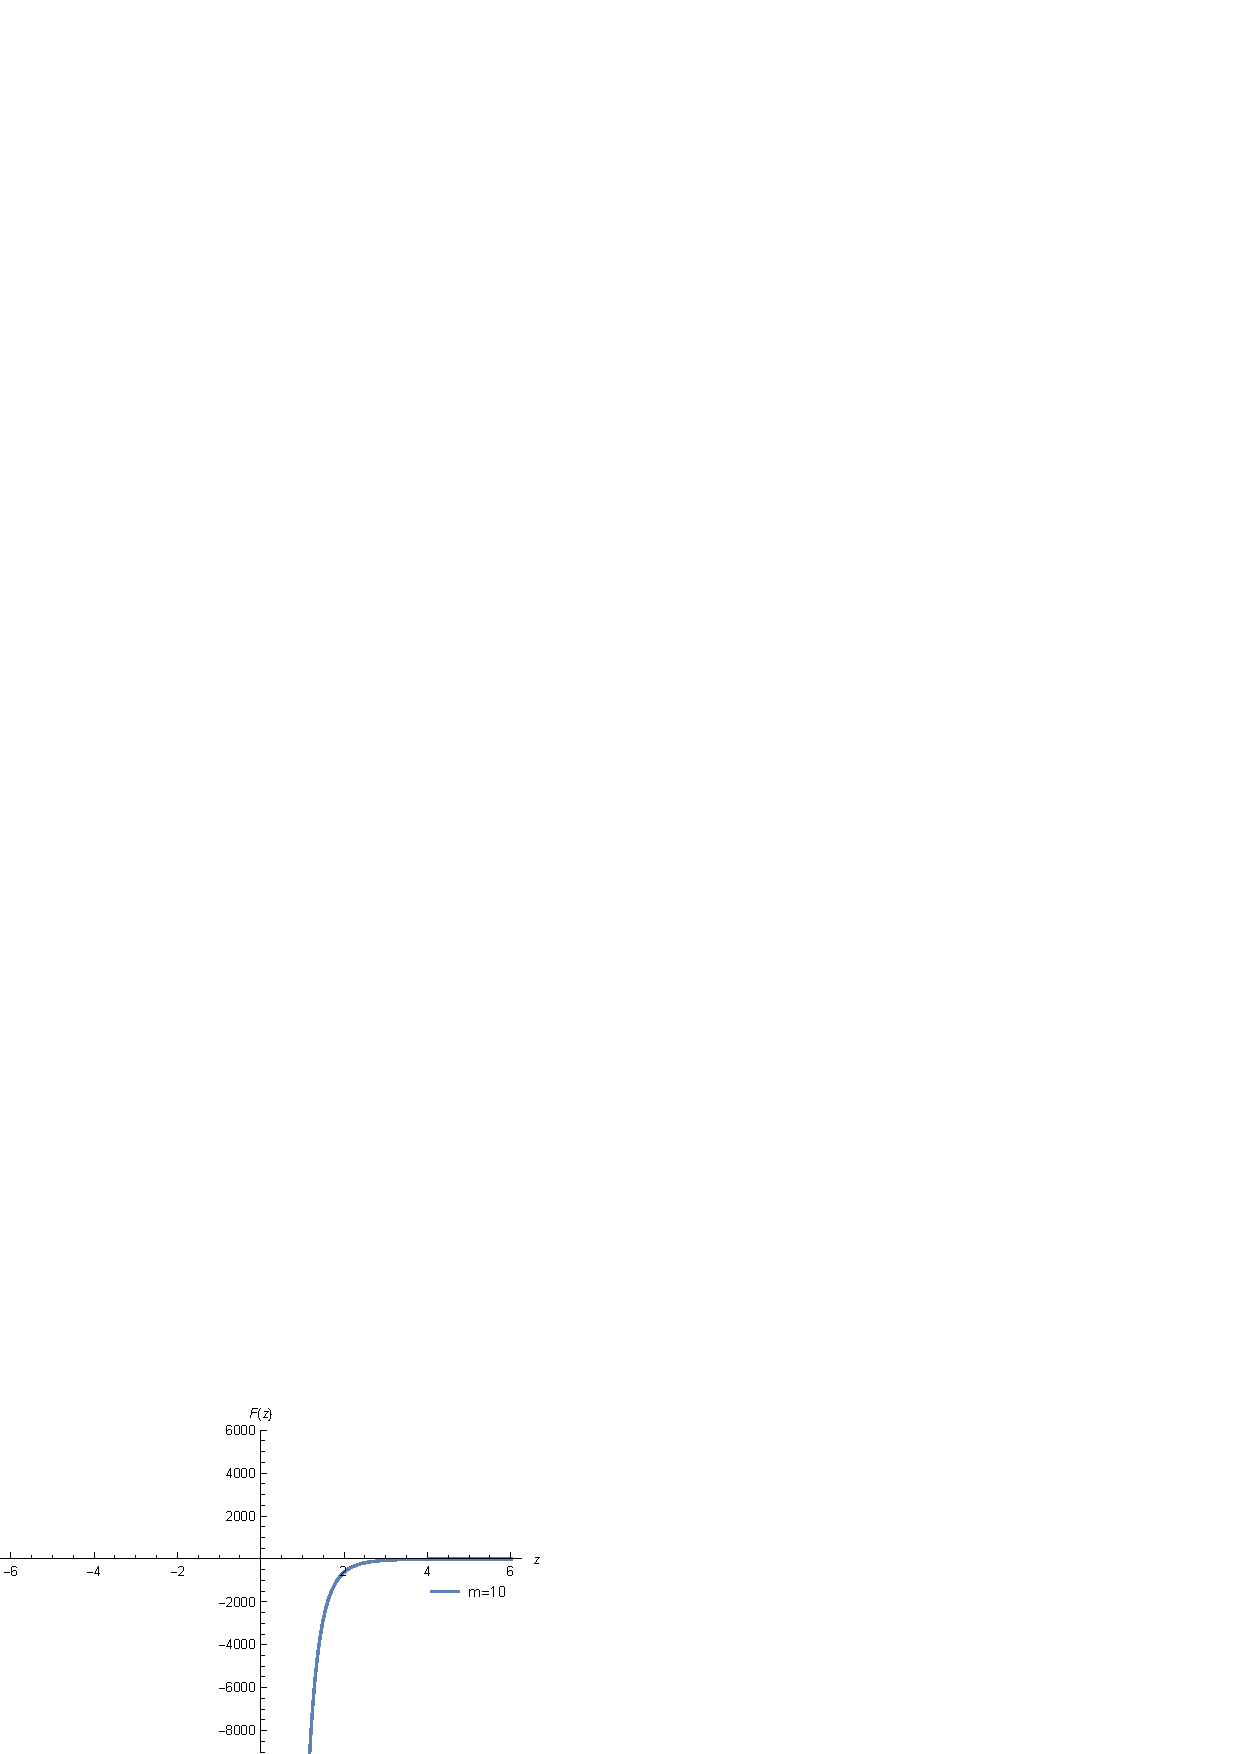
\includegraphics[width = 2.7in]{p10_F.pdf}}
\subfloat[]{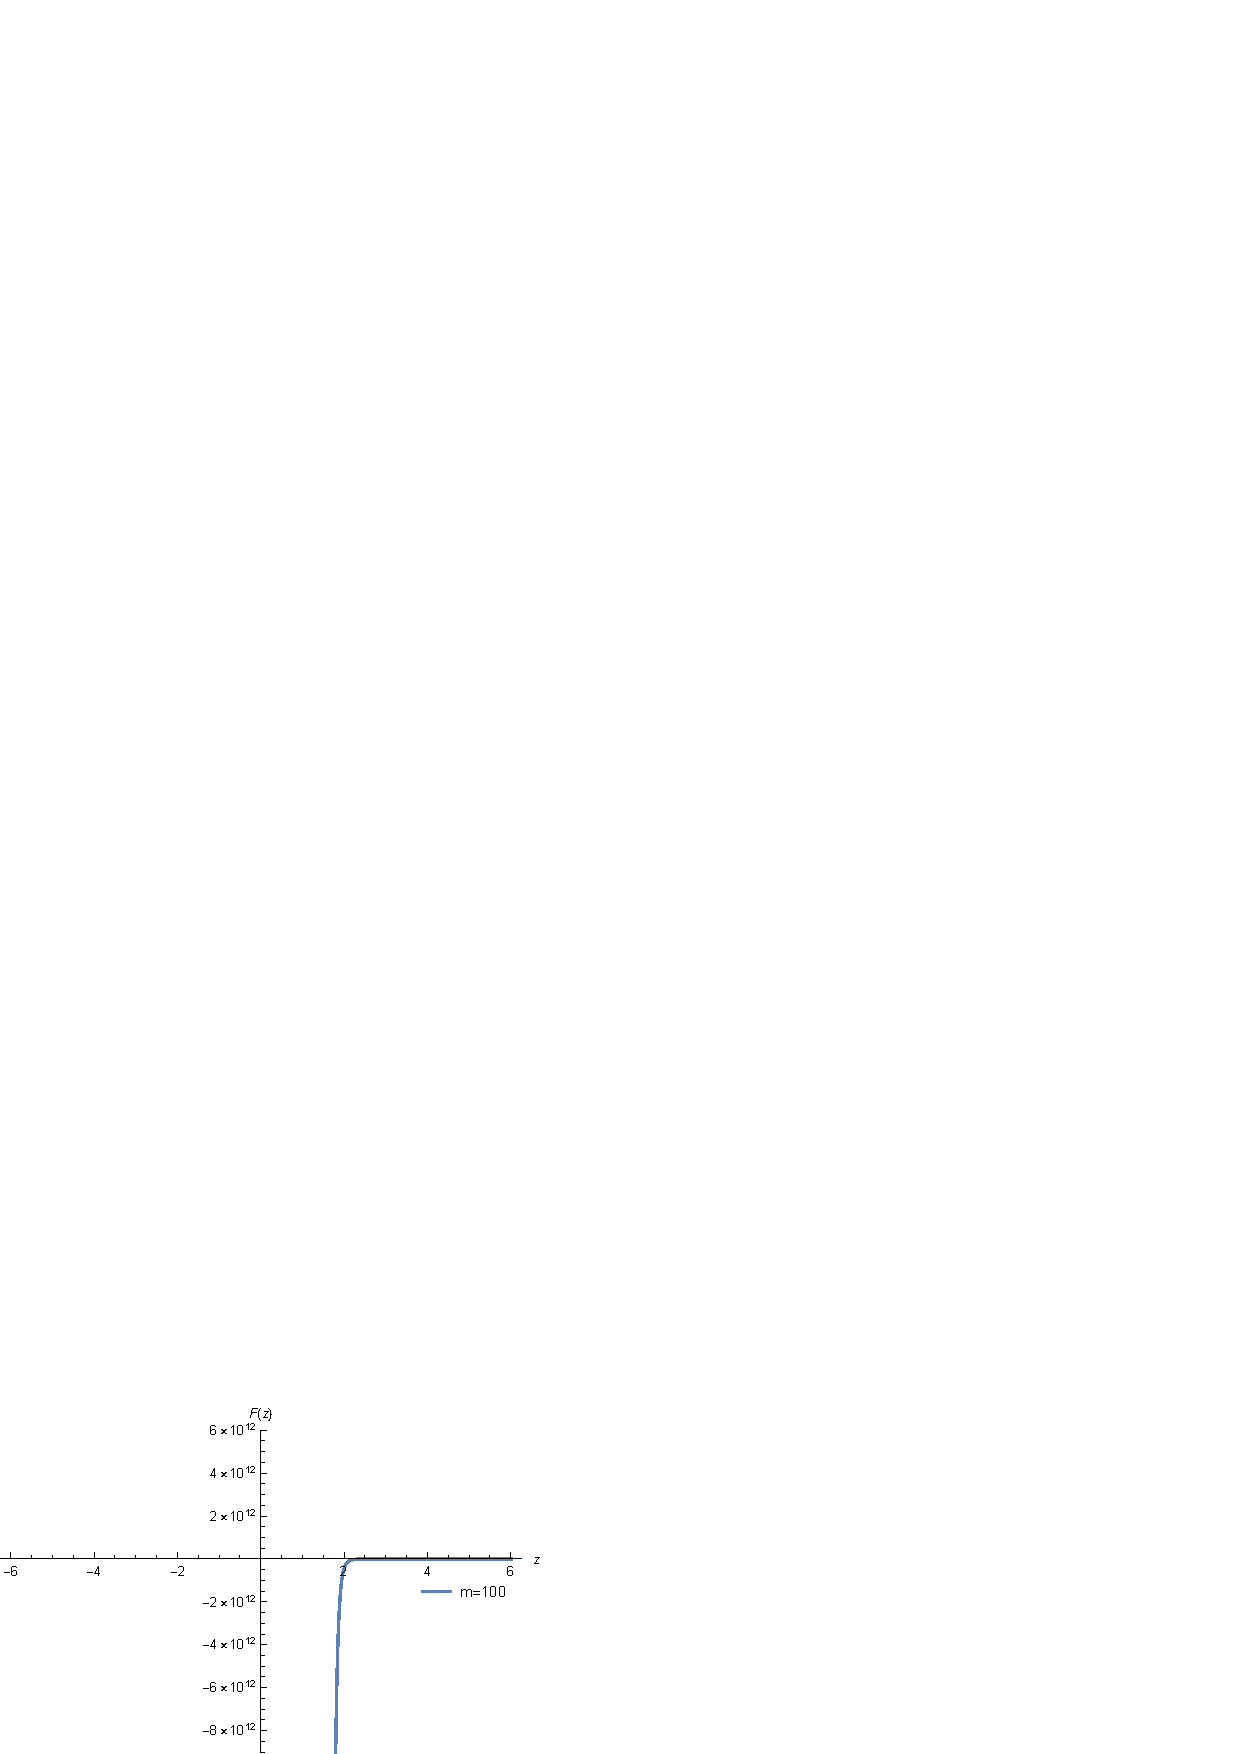
\includegraphics[width = 2.7in]{p100_F.pdf}} 
\caption{$F(z)$ for skewed logit model, z:[-6,6], m= 0.08, 0.18, 0.2,1,10, and 100}
\label{fig:skewedlogit_after_F}
\end{figure} Figures~\ref{fig:skewedlogit_after}-\ref{fig:skewedlogit_after_F} demonstrate $f_{4,4}(z)$ and $F(z)$ after use of ancillary functions for $m = 0.08, 0.18,$ $ 0.2, 1, 10$, and $100$. For $m\ge0.2$, both $f_{4,4}(z)$ and $F(z)$ do not intersect the horizontal axis, which validate the assumptions.
Unfortunately, we are not able to provide analytical proof of this result. The behavior of $f_{4,4}(z)$ and $F(z)$ for $m\in(0,0.2)$ remains to be resolved with more advanced tools. 


%While we cannot analytically prove that the  $F(z)=0$ does not have solution for $z\in (-\infty,\infty)$, we plot the $F(z)$ surface with Mathematica and observe that the surface remains below $F(z)=0$ (see Figure~\ref{fig:skewedlogit_after}). As a result, with the speculation $F(z)<0$ for $z\in (-\infty,\infty)$, the assumptions are satisfied. 

As a result of this speculation, we have $F(z)<0$ for $z\in (-\infty,\infty)$ when $m\ge 0.2$, and the assumptions are satisfied. Applying Theorem~\ref{2012a}, we know that considering $z\in[L,U]$ for any large $L<0$ and $U$, the designs with at most 3 support points including $U$ form a complete class. Further more, since this model is a Type III model with 2 parameters, through Theorem~\ref{removepts}, there always exists a complete class of 2 support points that contains the optimal design for $m\ge0.2$. The conclusions are summarized in Conjecture~
\ref{skew}.
% \begin{multline*}
%      -f_{4,4} = e^{-z} \left(3 (m-1) m e^{-2 z} \left(2 e^z \left(e^z+1\right)+2 e^{2 z}\right) \left(e^{-z}+1\right)^{m-2}+3 m e^{-z} \left(2 e^z \left(e^z+1\right)+2 e^{2 z}\right) \left(e^{-z}+1\right)^{m-1}-4 m e^{-z} \left(2 e^z \left(e^z+1\right)+6 e^{2 z}\right) \left(e^{-z}+1\right)^{m-1}+\left(2 e^z \left(e^z+1\right)+14 e^{2 z}\right) \left(\left(e^{-z}+1\right)^m-1\right)+6 e^{2 z} \left((m-1) m e^{-2 z} \left(e^{-z}+1\right)^{m-2}+m e^{-z} \left(e^{-z}+1\right)^{m-1}\right)+6 e^z \left(e^z+1\right) \left((m-1) m e^{-2 z} \left(e^{-z}+1\right)^{m-2}+m e^{-z} \left(e^{-z}+1\right)^{m-1}\right)+\left(e^z+1\right)^2 \left((m-3) (m-2) (m-1) m e^{-4 z} \left(e^{-z}+1\right)^{m-4}+6 (m-2) (m-1) m e^{-3 z} \left(e^{-z}+1\right)^{m-3}+7 (m-1) m e^{-2 z} \left(e^{-z}+1\right)^{m-2}+m e^{-z} \left(e^{-z}+1\right)^{m-1}\right)+8 e^z \left(e^z+1\right) \left((m-2) (m-1) m \left(-e^{-3 z}\right) \left(e^{-z}+1\right)^{m-3}-3 (m-1) m e^{-2 z} \left(e^{-z}+1\right)^{m-2}-m e^{-z} \left(e^{-z}+1\right)^{m-1}\right)\right)\\-e^{-z} \left(-3 m e^{-z} \left(2 e^z \left(e^z+1\right)+2 e^{2 z}\right) \left(e^{-z}+1\right)^{m-1}+\left(2 e^z \left(e^z+1\right)+6 e^{2 z}\right) \left(\left(e^{-z}+1\right)^m-1\right)+6 e^z \left(e^z+1\right) \left((m-1) m e^{-2 z} \left(e^{-z}+1\right)^{m-2}+m e^{-z} \left(e^{-z}+1\right)^{m-1}\right)+\left(e^z+1\right)^2 \left((m-2) (m-1) m \left(-e^{-3 z}\right) \left(e^{-z}+1\right)^{m-3}-3 (m-1) m e^{-2 z} \left(e^{-z}+1\right)^{m-2}-m e^{-z} \left(e^{-z}+1\right)^{m-1}\right)\right)
% \end{multline*}

     

\begin{conjecture}\label{skew}
For two parameter skewed logit model\[
P(y=1|x,\alpha,\beta) = \eta(x,\alpha,\beta)= \frac{1}{(1+e^{-\beta(x-\alpha)})^m}.
\]with a skewness parameter $m\ge0.2$, and $x\in (-\infty,+\infty)$. The designs with at most 2 points form a complete class.
\end{conjecture}



Conjecture~\ref{skew} provides a complete class of minimally supported designs for two-parameter skewed logit model. This complete class contains the optimal design in terms of Loewner Ordering. A similar result is provided by \cite{biedermann2006} which used the geometric approach to show that $\Phi_p$ optimal design for skewed logit model contains two support points for $m>0$. 



\section{Discussion}\label{dis}
In this paper, we proposed a tool called ancillary functions to identify optimal designs for nonlinear models, which extends the complete class strategy in \cite{yang2010} and \cite{yang2012} to more nonlinear models. While the use of ancillary functions may lead to more support points in the optimal design, our result shows that added support points are asymptotically removable under certain circumstances which makes minimally supported designs available for more nonlinear models that were not feasible with previous strategies. The results facilitate a more refined and unified framework for optimal designs for nonlinear models that simplify the mathematical derivation and numerical search.



The identification of minimally supported designs provides guidance in the search of an optimal design: A design with a larger support than the theoretical minimal support $n$ in the numerical search guides us to proceed with the search until a minimally supported design is found. Additionally, the resulting minimally supported design could be favorable in certain scenarios.
For example, in the manufacture industry, fewer support points in experimental design indicate fewer product prototypes, which induce less experimental cost since the production of a new prototype is often much more expensive than a replicate of an existing prototype.  In case of a big data scenario when direct model fitting is infeasible, this framework could help identify a most informative subset for efficient parameter estimation.

 
% The identification of minimally supported designs tremendously scales down the complexity in numerical search, and a minimally supported design could be favorable in certain scenarios. 







%  We provided an extension to the strategy in \cite{yang2010} and \cite{yang2012} to identify a complete class of designs for nonlinear models. We provide a resolution based on ancillary function when assumptions of Theorem~\ref{2012a} do not hold. We also showed that the added support points due to the newly added ancillary function could be removed from the final design for some models. We demonstrated our strategy with the Beta-Poisson model, the Complementary log-log model, and the Skewed logit model and obtained complete classes of minimally supported optimal designs, which were not feasible with previous strategies. With this strategy, we can identify a complete class of designs that contains the optimal design for more nonlinear models.
 
%  (how this result is better than others; what this method does for this area)
 
 
There are a few topics that we did not address adequately. In the three models explored - the Beta-Poisson model, complementary log-log model, and skewed logit model - we selected some shared factors of the $\Psi(z)$ functions in the sequence as the ancillary functions, yet we didn't give a general guide on how to make the selection. The scheme of the selection remains to be discussed in future work. Additionally in Section~\ref{secskew}, due to the complexity of skewed logit model, we did not provide a theoretical proof of $F(z)<0$ but instead used a numerical check through Mathematica for $m>0.2$. Interested readers could explore the analytical proof of Conjecture~\ref{skew}. More advanced tools are also called for to investigate the behavior of skewed logit model for $m\in (0,0.2)$. Last but not least, our strategy and conclusions in this paper currently only apply for information-based criteria. 




% Although we didn't give a general guide on how to select the ancillary functions, we do encourage our readers to experiment with functions related to the existing sequence. 
% We do not have a full arsenal of ancillary functions yet. 



%However, there are cases when parameters are estimated through other loss functions including exponential loss or Huber loss, in which case the Fisher information may not be an appropriate characterizing target. 
 
 
%  (what's next)
 
%  (so what + strong conclusions)


 
\nocite{*}
%\bibliographystyle{plain}
\bibliographystyle{apalike}
% \bibliography{ACM-Reference-Format}
\bibliography{bib_t} 
\end{document} 